\section{Basic System Properties}

\begin{frame}{Systems with and without Memory}
    A systems is said to be \alert{memoryless}  if its output for each value of the independent variable at a given time is dependent only on the input at the same time.
    \vspace{0.1in}
    \par
    \begin{columns}
        \column{0.48\textwidth}
            \textbf{Examples of memoryless systems}\par
            \begin{equation*}
                y[n] = (2x[n] - x^2[n])^2,
            \end{equation*}
            \begin{equation*}
                y(t) = Rx(t),
            \end{equation*}
            where $x(t)$ current through the resistor $R$ and $y(t)$ taken as the voltage across the resistor.
            \begin{equation*}
                y(t) = x(t),
            \end{equation*}
            which is called the \alert{identity system}. In DT
            \begin{equation*}
                y[n] = x[n].
            \end{equation*}
        \column{0.48\textwidth}
            \textbf{Examples of systems with memory}\par
            Accumulator or summer:
            \begin{equation*}
                y[n] = \sum_{k=-\infty}^{\infty}x[k].
            \end{equation*}
            Delay:
            \begin{equation*}
                y[n] = x[n-1].
            \end{equation*}
            Capacitor with current as the input and the output taken as the voltage:
            \begin{equation*}
                y(t) = \frac{1}{C}\int_{-\infty}^{t}x(\tau)d\tau.
            \end{equation*}
    \end{columns}
    \pause
    \mode<beamer>
    {
        \begin{tikzpicture}[remember picture,overlay]
            \node[anchor=east, yshift=-0.2in, fill=orange, opacity=.8,text opacity=1] at (current page.east)
            {$y[n] = \sum_{k=-\infty}^{n-1}x[k] + x[n], \quad y[n] = y[n-1] + x[n]$};
        \end{tikzpicture}
    }
\end{frame}


\begin{frame}{Invertibility and Inverse Systems}
    A system is \alert{invertible} of different inputs lead to difference outputs. If a system is invertible, the  an \alert{inverse system} exists, and when cascaded with the original system, yields an output equal to the input to the first system.
    \vspace{0.1in}
    \par
    \mode<beamer>
    {
        \centering
        \begin{tikzpicture}[node distance=4cm]
            \node (a) at (0,0) {$x[n]$};
            \node (b) [right= 1cm of a, thick, draw=Brown, fill=BurlyWood] {System};
            \node (c) [right= 1cm of b, thick, draw=Brown, fill=BurlyWood, text width=2cm, text centered] {Inverse system};
            \node (d) [right= 1cm of c] {$w[n] = x[n]$};
            \draw[-latex, thick, Brown] (a) -- (b);
            \draw[-latex, thick, Brown, text=black] (b) -- (c) node[midway, above] {$y[n]$};
            \draw[-latex, thick, Brown] (c) -- (d);
        \end{tikzpicture}
    }
    \mode<handout>
    {
        \vspace{0.5in}
    }
    \begin{columns}
        \column{0.48\textwidth}
        \textbf{ Examples of invertible systems:}\par
        If
        $
            y(t) = 2x(t),
        $
        the inverse system is
        \begin{equation*}
            w(t) = \frac{1}{2}y(t),
        \end{equation*}

        If (accumulator)
        $
                y[n] = \sum_{k=-\infty}^{\infty}x[k].
        $
            the inverse system is
        \begin{equation*}
            w[n] = y[n] - y[n-1].
        \end{equation*}
        \column{0.48\textwidth}
        \textbf{ Examples of non-invertible systems:}\par
        \begin{equation*}
            y[n] = 0.
        \end{equation*}
        \begin{equation*}
            y(t) = x^2(t).
        \end{equation*}
    \end{columns}
\end{frame}



\begin{frame}{Causality}
    A system is said to be causal if it only responds when you ``kick it.'' It response at any time depends only on that input prior or equal to that time. The system cannot anticipate future inputs.

    \begin{columns}
        \column{0.48\textwidth}
            \begin{align*}
              x_1(t) &\rightarrow y_1(t) \\
              x_2(t) &\rightarrow y_2(t) \\
            \end{align*}
            If
            \begin{equation*}
                x_1(t) = x_2(t) , \quad t < t_0,
            \end{equation*}
            then
            \begin{equation*}
                y_1(t) = y_2(t) , \quad t < t_0.
            \end{equation*}
            If inputs are identical until $t_0$, the outputs are identical until $t_0$. Same for DT.
        \column{0.48\textwidth}
        \textbf{ Example}
    \end{columns}
\end{frame}

\begin{frame}{Stability}
    Many forms. We choose Bounded Input Bounded Output (BIBO) stability.\par
    If a system is stable in BIBO sense, for every bounded input the output is bounded.
    \mode<beamer>
    {
        \begin{columns}
            \column{0.48\textwidth}
            \textbf{ Example}\par
            \begin{equation*}
                y(t) = \int_{-\infty}^{t}x(\tau)d\tau
            \end{equation*}
            is not stable.
            \column{0.48\textwidth}
        \end{columns}
    }
\end{frame}

\begin{frame}{Time Invariance}
    The system does not really care what we call the origin. If the input is shifted by any amount of time $t_0$, the output is also shifted by the same amount of time.
    \mode<beamer>
    {
        \begin{columns}
            \column{0.48\textwidth}
            If
            \begin{equation*}
                x(t) \rightarrow y(t),
            \end{equation*}
            then
            \begin{equation*}
                x(t - t_0) \rightarrow y(t - t_0).
            \end{equation*}

            If
            \begin{equation*}
                x[n] \rightarrow y[n],
            \end{equation*}
            then
            \begin{equation*}
                x[n - n_0] \rightarrow y[n - n_0].
            \end{equation*}
            \pause
            \column{0.48\textwidth}
            \textbf{ Example}\par
            Accumulator:
            \begin{equation*}
                y[n] = \sum_{k=-\infty}^{n}x[k]
            \end{equation*}
            \textbf{ Example}\par
            Modulator:
            \begin{equation*}
                y(t) = (\sin(t)x(t)
            \end{equation*}
        \end{columns}
    }
\end{frame}


\begin{frame}{Linearity}
    If
    \begin{align*}
      x_1(t) &\rightarrow y_1(t) \\
      x_2(t) &\rightarrow y_2(t) \\
    \end{align*}
    then
    \begin{equation*}
        ax_1(t) + bx_2(t) \rightarrow  ay_1(t) + by_2(t)
    \end{equation*}
    If the system is linear, if we give a linear combination of inputs, the output will allose be a similar linear combination of the original outputs.
    \mode<beamer>
    {
        \begin{columns}
            \column{0.48\textwidth}
            \column{0.48\textwidth}
        \end{columns}
    }
\end{frame}




\begin{frame}{Linear Time-Invariant Systems}
    \begin{enumerate}
        \item Systems that are both linear and time invariant are called Linear Time-Invariant (LTI) systems.
        \item With systems that are linear and time invariant, using the impulse function in CT and DT, produces an important and useful mechanism for characterizing those system.
        \item In this lecture we develop in detail the representation of both continuous-time and discrete-time signals as a linear combination of delayed impulses and the consequences for representing linear, time-invariant systems.
        \item The resulting representation is referred to as convolution.
    \end{enumerate}
\end{frame}


\section{Convolution}

\begin{frame}{Introduction (From Oppenheim)}
    \begin{itemize}
        \item A linear system: the response to a linear combination of inputs is the same linear combination of the individual responses.
        \item Time invariance: the system is not sensitive to the time origin. If the input is shifted in time by some amount, then the output is simply shifted by the same amount.
        \item For a linear system, if the system inputs can be decomposed as a linear combination of some basic inputs and the system response is known for each of the basic inputs, then the response can be constructed as the same linear combination of the responses to each of the basic inputs.
        \item Signals can be decomposed as a linear combination of basic signals in a variety of ways (e.g., Taylor series expansion that expresses a function in polynomial form.) However, in the context of signals and systems, it is important to choose the basic signals in the expansion so that in some sense the response is easy to compute.
        \item For systems that are both linear and time-invariant, there are two particularly useful choices for these basic signals: delayed impulses and complex exponentials.
    \end{itemize}
\end{frame}

\begin{frame}{Introduction (From Oppenheim)}
    \begin{itemize}
        \item In this lecture we develop in detail the representation of both continuous-time and discrete-time signals as a linear combination of delayed impulses and the consequences for representing linear, time-invariant systems. The resulting representation is referred to as convolution.
        \item Earlier, we developed in detail the decomposition of signals as linear combinations of complex exponentials (referred to as Fourier analysis) and the consequence of that representation for linear, time-invariant systems.
    \end{itemize}
\end{frame}

\begin{frame}{Introduction}
    \begin{itemize}
        \item Using the convolution we can express the response of an LTI system to an arbitrary input in terms of the system's response to the unit impulse.
        \item An LTI system is completely characterized by its response to a single signal, namely, its response to the unit impulse.
        \item In discrete time, we have the convolution sum. In continuous time, we have the convolution integral.
    \end{itemize}
\end{frame}

\begin{frame}{Strategy for Exploiting Linearity and Time Invariance}
    \mode<beamer>
    {
    \begin{itemize}
        \item Decompose the input signal to a linear combination of basic signals.
        \item   Chose basic signals so that the response is easy to compute (analytical convenience).
    \end{itemize}

    \begin{enumerate}
        \item Delayed impulses $\rightarrow$ convolution
        \item Complex exponentials $\rightarrow$ Fourier analysis
    \end{enumerate}
    }
\end{frame}


%%%%%%%%%%%%%%%%%%%%%%%%%%%%%%%%%%%%%%%%%%%%%
\subsection{The Discrete-Time Unit Impulse Response and the Convolution Sum}

\begin{frame}{A DT Signal as  Superposition of Weighted Delayed Impulses}
    \begin{itemize}
      \item We can express a DT signal as a linear combination of weighted delayed impulses.
      \item If we have a liner system, and a signal expressed as above as a linear combination of basic signals, the response would be the same linear combinaton fo the responses for individual basic signals.
    \end{itemize}

\end{frame}


\begin{frame}[plain]
    \mode<beamer>
    {
        \begin{columns}
            \column{0.48\textwidth}
                \begin{figure}
                  \centering
                  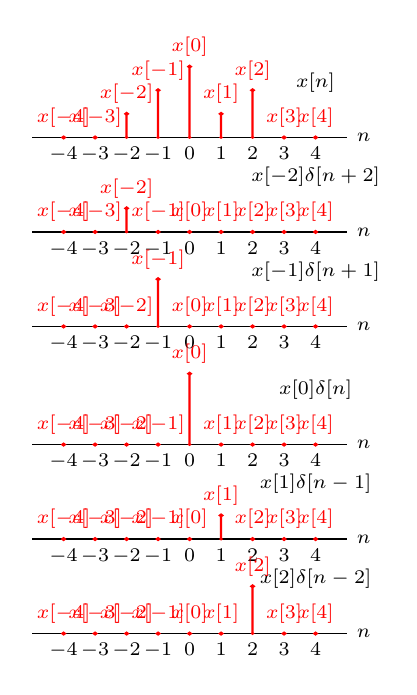
\begin{tikzpicture}[xscale=0.4, yscale=0.3, every label/.append style={text=black}]

	\def\nmin{-4}
	\def\nmax{4}	
	
		
	\begin{scope}	
		\def\x{{0, 0, 1, 2, 3, 1, 2, 0, 0}}		
		\draw (\nmin-1, 0) -- (\nmax+1,0) node[anchor=west] {\scriptsize $n$};
		\foreach \n in {\nmin, ..., \nmax}
		{
			\node at (\n, 0) [anchor=north] {\scriptsize $\n$};
		}
		\node at (\nmax,1.5) [anchor=south] {\scriptsize $x[n]$};
		
		\foreach \n/\a in {0/{-4},1/{-3}, 2/{-2}, 3/{-1}, 4/{0}, 5/{1}, 6/{2}, 7/{3}, 8/{4}}
		{
			\pgfmathparse{\x[\n]}
			\edef\xn{\pgfmathresult}	
			\ifthenelse{\xn > 0}
			{

				\draw[red, thick, fill=red]  (\n + \nmin, 0) -- ++(0, \xn) circle (1pt) node[anchor=south] {\scriptsize $x[\a]$};
			}
			{
				\draw[red, fill=red] (\n+ \nmin,  0) circle (1pt);
			}
		}
	\end{scope}	
	
	\pause
	
	\begin{scope}[yshift=-4cm]
		\def\x{{0, 0, 1, 0, 0, 0, 0, 0, 0}}		
		\draw (\nmin-1, 0) -- (\nmax+1,0) node[anchor=west] {\scriptsize $n$};
		\foreach \n in {\nmin, ..., \nmax}
		{
			\node at (\n, 0) [anchor=north] {\scriptsize $\n$};
		}
		\node at (\nmax,1.5) [anchor=south] {\scriptsize $x[-2]\delta[n+2]$};
		
		\foreach \n/\a in {0/{-4},1/{-3}, 2/{-2}, 3/{-1}, 4/{0}, 5/{1}, 6/{2}, 7/{3}, 8/{4}}
		{
			\pgfmathparse{\x[\n]}
			\edef\xn{\pgfmathresult}	
			\ifthenelse{\xn > 0}
			{

				\draw[red, thick, fill=red]  (\n + \nmin, 0) -- ++(0, \xn) circle (1pt) node[anchor=south] {\scriptsize $x[\a]$};
			}
			{
				\draw[red, fill=red] (\n+ \nmin,  0) circle (1pt);
			}
		}
	\end{scope}		

	\pause

	\begin{scope}[yshift=-8cm]
		\def\x{{0, 0, 0, 2, 0, 0, 0, 0, 0}}		
		\draw (\nmin-1, 0) -- (\nmax+1,0) node[anchor=west] {\scriptsize $n$};
		\foreach \n in {\nmin, ..., \nmax}
		{
			\node at (\n, 0) [anchor=north] {\scriptsize $\n$};
		}
		\node at (\nmax,1.5) [anchor=south] {\scriptsize $x[-1]\delta[n+1]$};
		
		\foreach \n/\a in {0/{-4},1/{-3}, 2/{-2}, 3/{-1}, 4/{0}, 5/{1}, 6/{2}, 7/{3}, 8/{4}}
		{
			\pgfmathparse{\x[\n]}
			\edef\xn{\pgfmathresult}	
			\ifthenelse{\xn > 0}
			{

				\draw[red, thick, fill=red]  (\n + \nmin, 0) -- ++(0, \xn) circle (1pt) node[anchor=south] {\scriptsize $x[\a]$};
			}
			{
				\draw[red, fill=red] (\n+ \nmin,  0) circle (1pt);
			}
		}
	\end{scope}		
	
	\pause	
%	
	\begin{scope}[yshift=-13cm]
		\def\x{{0, 0, 0, 0, 3, 0, 0, 0, 0}}		
		\draw (\nmin-1, 0) -- (\nmax+1,0) node[anchor=west] {\scriptsize $n$};
		\foreach \n in {\nmin, ..., \nmax}
		{
			\node at (\n, 0) [anchor=north] {\scriptsize $\n$};
		}
		\node at (\nmax,1.5) [anchor=south] {\scriptsize $x[0]\delta[n]$};
		
		\foreach \n/\a in {0/{-4},1/{-3}, 2/{-2}, 3/{-1}, 4/{0}, 5/{1}, 6/{2}, 7/{3}, 8/{4}}
		{
			\pgfmathparse{\x[\n]}
			\edef\xn{\pgfmathresult}	
			\ifthenelse{\xn > 0}
			{

				\draw[red, thick, fill=red]  (\n + \nmin, 0) -- ++(0, \xn) circle (1pt) node[anchor=south] {\scriptsize $x[\a]$};
			}
			{
				\draw[red, fill=red] (\n+ \nmin,  0) circle (1pt);
			}
		}
	\end{scope}		
	
	\pause	
	
	\begin{scope}[yshift=-17cm]
		\def\x{{0, 0, 0, 0, 0, 1, 0, 0, 0}}		
		\draw (\nmin-1, 0) -- (\nmax+1,0) node[anchor=west] {\scriptsize $n$};
		\foreach \n in {\nmin, ..., \nmax}
		{
			\node at (\n, 0) [anchor=north] {\scriptsize $\n$};
		}
		\node at (\nmax,1.5) [anchor=south] {\scriptsize $x[1]\delta[n-1]$};
		
		\foreach \n/\a in {0/{-4},1/{-3}, 2/{-2}, 3/{-1}, 4/{0}, 5/{1}, 6/{2}, 7/{3}, 8/{4}}
		{
			\pgfmathparse{\x[\n]}
			\edef\xn{\pgfmathresult}	
			\ifthenelse{\xn > 0}
			{

				\draw[red, thick, fill=red]  (\n + \nmin, 0) -- ++(0, \xn) circle (1pt) node[anchor=south] {\scriptsize $x[\a]$};
			}
			{
				\draw[red, fill=red] (\n+ \nmin,  0) circle (1pt);
			}
		}
	\end{scope}		
	
	\pause	

%
	\begin{scope}[yshift=-21cm]
		\def\x{{0, 0, 0, 0, 0, 0, 2, 0, 0}}		
		\draw (\nmin-1, 0) -- (\nmax+1,0) node[anchor=west] {\scriptsize $n$};
		\foreach \n in {\nmin, ..., \nmax}
		{
			\node at (\n, 0) [anchor=north] {\scriptsize $\n$};
		}
		\node at (\nmax,1.5) [anchor=south] {\scriptsize $x[2]\delta[n-2]$};
		
		\foreach \n/\a in {0/{-4},1/{-3}, 2/{-2}, 3/{-1}, 4/{0}, 5/{1}, 6/{2}, 7/{3}, 8/{4}}
		{
			\pgfmathparse{\x[\n]}
			\edef\xn{\pgfmathresult}	
			\ifthenelse{\xn > 0}
			{

				\draw[red, thick, fill=red]  (\n + \nmin, 0) -- ++(0, \xn) circle (1pt) node[anchor=south] {\scriptsize $x[\a]$};
			}
			{
				\draw[red, fill=red] (\n+ \nmin,  0) circle (1pt);
			}
		}
	\end{scope}		
	
	
\end{tikzpicture}


                  \caption{}\label{fi:dt_as_superposition}
                \end{figure}
            \column{0.48\textwidth}
            \pause
            \begin{align*}
              x[n] &= x[-2]\delta[n+2] \\
              &  x[-1]\delta[n+1] \\
              &  x[0]\delta[n] \\
              &  x[1]\delta[n-1] \\
              &  x[2]\delta[n-2] \\
              x[n] &= \sum_{k=-\infty}^{\infty}x[k]\delta[n-k].
            \end{align*}
            A linear combination of weighted delayed impulses.
        \end{columns}
    }
\end{frame}


\begin{frame}{Convolution Sum}
    \mode<beamer>
    {
    \begin{align*}
        x[n] &= \sum_{k=-\infty}^{\infty}x[k]\delta[n-k], \quad \text{input}.
    \end{align*}
    \pause
    Linear system
    \pause
    \begin{align*}
        y[n] &= \sum_{k=-\infty}^{\infty}x[k]h_k[n] \quad \text{where }h_k[n] \text{ is the output due to the delayed impulse}.\\
        \delta[n-k] &\rightarrow h_k[n].
    \end{align*}
    \pause
    If time invariant
    \pause
    \begin{align*}
        h_k[n] &= h_0[n-k] \quad \text{where }h_0 \text{ is the response of the system for an impulse at 0}.\\
        h_0[n] &= h[n] \quad \text{define}.
    \end{align*}
    \pause
    If LTI
    \begin{equation*}
        \boxed{y[n] = \sum_{k=-\infty}^{\infty}x[k]h[n-k]}\quad \text{convolution sum}.
    \end{equation*}

    }
\end{frame}




\begin{frame}{Convolution Sum: Summary}
    The convolution of the sequence $x[n]$ and $h[n]$ is given by
    \begin{equation}\label{eq:convolution_sum}
        y[n] = \sum_{k=-\infty}^{\infty}x[k]h[n-k],
    \end{equation}
    which we represent symbolically as
    \begin{equation}\label{eq:convolution_symbol}
        y[n] = x[n]\ast h[n]
    \end{equation}
\end{frame}


\begin{frame}{Example}
    Computer $y[n] = x[n]\ast h[n]$ for $x[n]$ and $h[n]$ as shown in Figure \ref{fi:example01_discrete_conv_signals}.
    \mode<beamer>
    {
    \begin{figure}
      \centering
      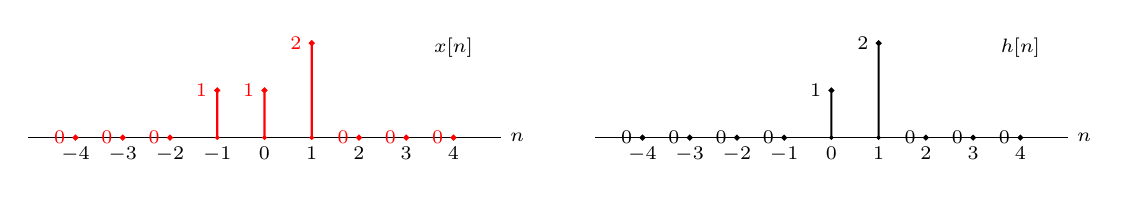
\begin{tikzpicture}[scale=0.6]

	\def\nmin{-4}
	\def\nmax{4}	
	
	\begin{scope}	
		\def\x{{0, 0, 0, 1, 1, 2, 0, 0, 0}}	

		\draw (\nmin-1, 0) -- (\nmax+1,0) node[anchor=west] {\scriptsize $n$};
		\foreach \n in {\nmin, ..., \nmax}
		{
			\node at (\n, 0) [anchor=north] {\scriptsize $\n$};
		}
		\node at (\nmax,1.5) [anchor=south] {\scriptsize $x[n]$};
		
		\foreach \n in {0,1, ...,8}
		{
			\pgfmathparse{\x[\n]}
			\edef\xn{\pgfmathresult}	
			\ifthenelse{\xn > 0}
			{
				\draw[red, thick, fill=red]  (\n + \nmin, 0) -- ++(0, \xn) circle (1pt) node[anchor=east] {\scriptsize $\xn$};
			}
			{
				\draw[red, fill=red] (\n+ \nmin,  0) circle (1pt);
			}
		}
	\end{scope}	
	
	\begin{scope}[xshift=12cm, yshift=0cm]	
		\def\h{{0, 0, 0, 0, 1, 2, 0, 0, 0}}	
		\draw (\nmin-1, 0) -- (\nmax+1,0) node[anchor=west] {\scriptsize $n$};
		\foreach \n in {\nmin, ..., \nmax}
		{
			\node at (\n, 0) [anchor=north] {\scriptsize $\n$};
		}
		\node at (\nmax,1.5) [anchor=south] {\scriptsize $h[n]$};
		
		\foreach \n in {0,1, ...,8}
		{
			\pgfmathparse{\h[\n]}
			\edef\hn{\pgfmathresult}	
			\ifthenelse{\hn > 0}
			{
				\draw[thick, fill=black]  (\n + \nmin, 0) -- ++(0, \hn) circle (1pt) node[anchor=east] {\scriptsize $\hn$};
			}
			{
				\draw[fill=black] (\n+ \nmin,  0) circle (1pt);
			}
		}
	\end{scope}		
	

\end{tikzpicture}


      \caption{Computing convolution}\label{fi:example01_discrete_conv_signals}
    \end{figure}
    }
\end{frame}

\begin{frame}<beamer>[plain,t]
    \mode<beamer>
    {
    \begin{figure}
      \centering
      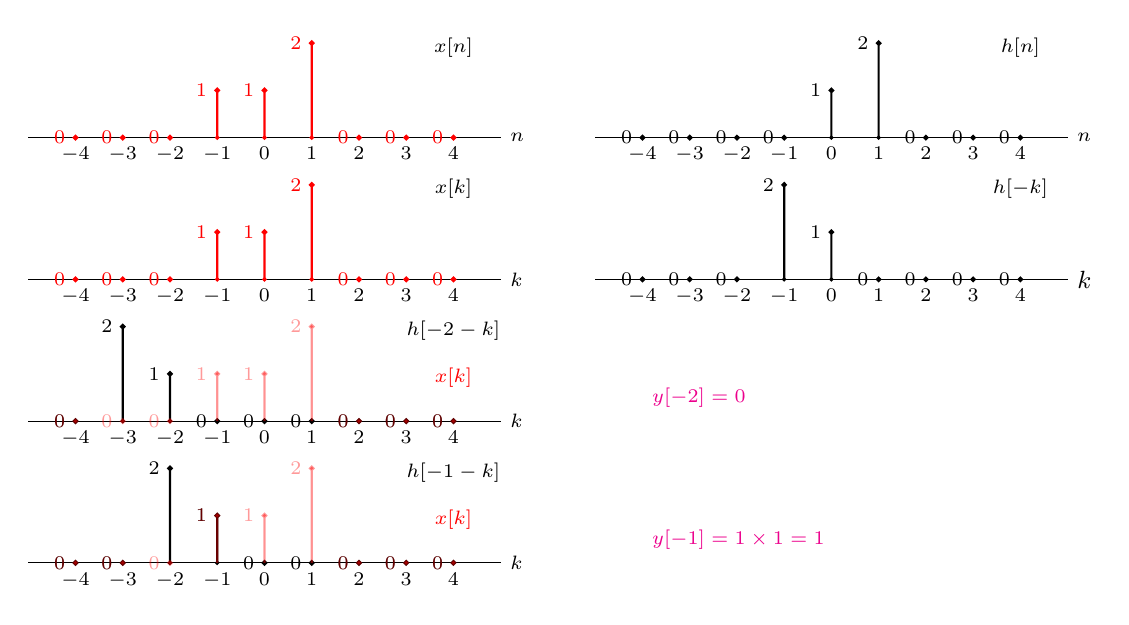
\begin{tikzpicture}[scale=0.6]

	\def\nmin{-4}
	\def\nmax{4}	
	
	\begin{scope}	
		\def\x{{0, 0, 0, 1, 1, 2, 0, 0, 0}}	

		\draw (\nmin-1, 0) -- (\nmax+1,0) node[anchor=west] {\scriptsize $n$};
		\foreach \n in {\nmin, ..., \nmax}
		{
			\node at (\n, 0) [anchor=north] {\scriptsize $\n$};
		}
		\node at (\nmax,1.5) [anchor=south] {\scriptsize $x[n]$};
		
		\foreach \n in {0,1, ...,8}
		{
			\pgfmathparse{\x[\n]}
			\edef\xn{\pgfmathresult}	
			\ifthenelse{\xn > 0}
			{
				\draw[red, thick, fill=red]  (\n + \nmin, 0) -- ++(0, \xn) circle (1pt) node[anchor=east] {\scriptsize $\xn$};
			}
			{
				\draw[red, fill=red] (\n+ \nmin,  0) circle (1pt);
			}
		}
	\end{scope}	
	
	\begin{scope}[xshift=12cm, yshift=0cm]	
		\def\h{{0, 0, 0, 0, 1, 2, 0, 0, 0}}	
		\draw (\nmin-1, 0) -- (\nmax+1,0) node[anchor=west] {\scriptsize $n$};
		\foreach \n in {\nmin, ..., \nmax}
		{
			\node at (\n, 0) [anchor=north] {\scriptsize $\n$};
		}
		\node at (\nmax,1.5) [anchor=south] {\scriptsize $h[n]$};
		
		\foreach \n in {0,1, ...,8}
		{
			\pgfmathparse{\h[\n]}
			\edef\hn{\pgfmathresult}	
			\ifthenelse{\hn > 0}
			{
				\draw[thick, fill=black]  (\n + \nmin, 0) -- ++(0, \hn) circle (1pt) node[anchor=east] {\scriptsize $\hn$};
			}
			{
				\draw[fill=black] (\n+ \nmin,  0) circle (1pt);
			}
		}
	\end{scope}		
	
	\begin{scope}[xshift=0cm, yshift=-3cm]		
		\def\x{{0, 0, 0, 1, 1, 2, 0, 0, 0}}	

		\draw (\nmin-1, 0) -- (\nmax+1,0) node[anchor=west] {\scriptsize $k$};
		\foreach \n in {\nmin, ..., \nmax}
		{
			\node at (\n, 0) [anchor=north] {\scriptsize $\n$};
		}
		\node at (\nmax,1.5) [anchor=south] {\scriptsize $x[k]$};
		
		\foreach \n in {0,1, ...,8}
		{
			\pgfmathparse{\x[\n]}
			\edef\xn{\pgfmathresult}	
			\ifthenelse{\xn > 0}
			{
				\draw[red, thick, fill=red]  (\n + \nmin, 0) -- ++(0, \xn) circle (1pt) node[anchor=east] {\scriptsize $\xn$};
			}
			{
				\draw[red, fill=red] (\n+ \nmin,  0) circle (1pt);
			}
		}
	\end{scope}	
	
	\begin{scope}[xshift=12cm, yshift=-3cm]	
		\def\h{{0, 0, 0, 2, 1, 0, 0, 0, 0}}	
		\draw (\nmin-1, 0) -- (\nmax+1,0) node[anchor=west] {\small $k$};
		\foreach \n in {\nmin, ..., \nmax}
		{
			\node at (\n, 0) [anchor=north] {\scriptsize $\n$};
		}
		\node at (\nmax,1.5) [anchor=south] {\scriptsize $h[-k]$};
		
		\foreach \n in {0,1, ...,8}
		{
			\pgfmathparse{\h[\n]}
			\edef\hn{\pgfmathresult}	
			\ifthenelse{\hn > 0}
			{
				\draw[thick, fill=black]  (\n + \nmin, 0) -- ++(0, \hn) circle (1pt) node[anchor=east] {\scriptsize $\hn$};
			}
			{
				\draw[fill=black] (\n+ \nmin,  0) circle (1pt);
			}
		}
	\end{scope}		
	
	\begin{scope}[xshift=0cm, yshift=-6cm]	
		\def\h{{ 0, 2, 1, 0, 0, 0, 0, 0, 0}}		
		\draw (\nmin-1, 0) -- (\nmax+1,0) node[anchor=west] {\scriptsize $k$};
		\foreach \n in {\nmin, ..., \nmax}
		{
			\node at (\n, 0) [anchor=north] {\scriptsize $\n$};
		}
		\node at (\nmax,1.5) [anchor=south] {\scriptsize $h[-2-k]$};
		
		\foreach \n in {0,1, ...,8}
		{
			\pgfmathparse{\h[\n]}
			\edef\hn{\pgfmathresult}	
			\ifthenelse{\hn > 0}
			{
				\draw[thick, fill=black]  (\n + \nmin, 0) -- ++(0, \hn) circle (1pt) node[anchor=east] {\scriptsize $\hn$};
			}
			{
				\draw[fill=black] (\n+ \nmin,  0) circle (1pt);
			}
		}
	\end{scope}		
	
	\begin{scope}[xshift=0cm, yshift=-9cm]	
		\def\h{{ 0, 0, 2, 1, 0, 0, 0, 0, 0}}		
		\draw (\nmin-1, 0) -- (\nmax+1,0) node[anchor=west] {\scriptsize $k$};
		\foreach \n in {\nmin, ..., \nmax}
		{
			\node at (\n, 0) [anchor=north] {\scriptsize $\n$};
		}
		\node at (\nmax,1.5) [anchor=south] {\scriptsize $h[-1-k]$};
		
		\foreach \n in {0,1, ...,8}
		{
			\pgfmathparse{\h[\n]}
			\edef\hn{\pgfmathresult}	
			\ifthenelse{\hn > 0}
			{
				\draw[thick, fill=black]  (\n + \nmin, 0) -- ++(0, \hn) circle (1pt) node[anchor=east] {\scriptsize $\hn$};
			}
			{
				\draw[fill=black] (\n+ \nmin,  0) circle (1pt);
			}
		}
	\end{scope}	
	
    \pause
	
	\begin{scope}[xshift=0cm, yshift=-6cm]		
		\def\x{{0, 0, 0, 1, 1, 2, 0, 0, 0}}	


		\node at (\nmax,.5) [anchor=south, red] {\scriptsize $x[k]$};
		
		\foreach \n in {0,1, ...,8}
		{
			\pgfmathparse{\x[\n]}
			\edef\xn{\pgfmathresult}	
			\ifthenelse{\xn > 0}
			{
				\draw[red, thick, fill=red, opacity=.4]  (\n + \nmin, 0) -- ++(0, \xn) circle (1pt) node[anchor=east] {\scriptsize $\xn$};
			}
			{

			}
		}
	\end{scope}		
	
	
	\begin{scope}[xshift=0cm, yshift=-9cm]		
		\def\x{{0, 0, 0, 1, 1, 2, 0, 0, 0}}	


		\node at (\nmax,.5) [anchor=south, red] {\scriptsize $x[k]$};
		
		\foreach \n in {0,1, ...,8}
		{
			\pgfmathparse{\x[\n]}
			\edef\xn{\pgfmathresult}	
			\ifthenelse{\xn > 0}
			{
				\draw[red, thick, fill=red, opacity=.4]  (\n + \nmin, 0) -- ++(0, \xn) circle (1pt) node[anchor=east] {\scriptsize $\xn$};
			}
			{

			}
		}
	\end{scope}			
	
    \pause
	
	\begin{scope}[xshift=8cm, yshift=-6cm]		

		\node at (0,.5) [anchor=west, magenta] {\scriptsize $y[-2] = 0$};
		
	\end{scope}		
	
	
	\begin{scope}[xshift=8cm, yshift=-9cm]		
		\node at (0,.5) [anchor=west, magenta] {\scriptsize $y[-1] = 1\times 1 = 1 $};
	\end{scope}		
\end{tikzpicture}


      \caption{Computing convolution}\label{fi:example01_discrete_conv_01}
    \end{figure}
    }
\end{frame}

\begin{frame}<beamer>[plain,t]
    \mode<beamer>
    {
    \begin{figure}
      \centering
      
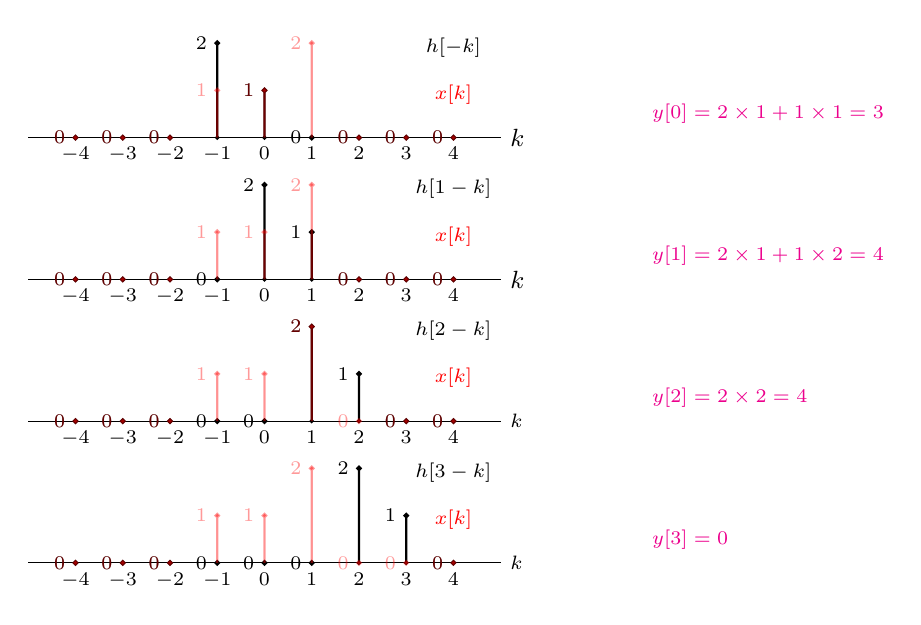
\begin{tikzpicture}[scale=0.6]
	\def\nmin{-4}
	\def\nmax{4}		
	\begin{scope}[xshift=0cm, yshift=0cm]	
		\def\h{{0,  0, 0, 2, 1, 0, 0, 0, 0}}		
		\draw (\nmin-1, 0) -- (\nmax+1,0) node[anchor=west] {\small $k$};
		\foreach \n in {\nmin, ..., \nmax}
		{
			\node at (\n, 0) [anchor=north] {\scriptsize $\n$};
		}
		\node at (\nmax,1.5) [anchor=south] {\scriptsize $h[-k]$};
		
		\foreach \n in {0,1, ...,8}
		{
			\pgfmathparse{\h[\n]}
			\edef\hn{\pgfmathresult}	
			\ifthenelse{\hn > 0}
			{
				\draw[thick, fill=black]  (\n + \nmin, 0) -- ++(0, \hn) circle (1pt) node[anchor=east] {\scriptsize $\hn$};
			}
			{
				\draw[fill=black] (\n+ \nmin,  0) circle (1pt);
			}
		}
	\end{scope}		


	\begin{scope}[xshift=0cm, yshift=-3cm]	
		\def\h{{0, 0,  0, 0, 2, 1, 0, 0, 0}}		
		\draw (\nmin-1, 0) -- (\nmax+1,0) node[anchor=west] {\small $k$};
		\foreach \n in {\nmin, ..., \nmax}
		{
			\node at (\n, 0) [anchor=north] {\scriptsize $\n$};
		}
		\node at (\nmax,1.5) [anchor=south] {\scriptsize $h[1-k]$};
		
		\foreach \n in {0,1, ...,8}
		{
			\pgfmathparse{\h[\n]}
			\edef\hn{\pgfmathresult}	
			\ifthenelse{\hn > 0}
			{
				\draw[thick, fill=black]  (\n + \nmin, 0) -- ++(0, \hn) circle (1pt) node[anchor=east] {\scriptsize $\hn$};
			}
			{
				\draw[fill=black] (\n+ \nmin,  0) circle (1pt);
			}
		}
	\end{scope}		


	\begin{scope}[xshift=0cm, yshift=-6cm]	
		\def\h{{0, 0, 0,  0, 0, 2, 1, 0, 0}}		
		\draw (\nmin-1, 0) -- (\nmax+1,0) node[anchor=west] {\scriptsize $k$};
		\foreach \n in {\nmin, ..., \nmax}
		{
			\node at (\n, 0) [anchor=north] {\scriptsize $\n$};
		}
		\node at (\nmax,1.5) [anchor=south] {\scriptsize $h[2-k]$};
		
		\foreach \n in {0,1, ...,8}
		{
			\pgfmathparse{\h[\n]}
			\edef\hn{\pgfmathresult}	
			\ifthenelse{\hn > 0}
			{
				\draw[thick, fill=black]  (\n + \nmin, 0) -- ++(0, \hn) circle (1pt) node[anchor=east] {\scriptsize $\hn$};
			}
			{
				\draw[fill=black] (\n+ \nmin,  0) circle (1pt);
			}
		}
	\end{scope}		
	
	\begin{scope}[xshift=0cm, yshift=-9cm]	
		\def\h{{0, 0, 0, 0,  0, 0, 2, 1, 0}}		
		\draw (\nmin-1, 0) -- (\nmax+1,0) node[anchor=west] {\scriptsize $k$};
		\foreach \n in {\nmin, ..., \nmax}
		{
			\node at (\n, 0) [anchor=north] {\scriptsize $\n$};
		}
		\node at (\nmax,1.5) [anchor=south] {\scriptsize $h[3-k]$};
		
		\foreach \n in {0,1, ...,8}
		{
			\pgfmathparse{\h[\n]}
			\edef\hn{\pgfmathresult}	
			\ifthenelse{\hn > 0}
			{
				\draw[thick, fill=black]  (\n + \nmin, 0) -- ++(0, \hn) circle (1pt) node[anchor=east] {\scriptsize $\hn$};
			}
			{
				\draw[fill=black] (\n+ \nmin,  0) circle (1pt);
			}
		}
	\end{scope}			

   \pause
	\begin{scope}[xshift=0cm, yshift=0cm]		
		\def\x{{0, 0, 0, 1, 1, 2, 0, 0, 0}}	


		\node at (\nmax,.5) [anchor=south, red] {\scriptsize $x[k]$};
		
		\foreach \n in {0,1, ...,8}
		{
			\pgfmathparse{\x[\n]}
			\edef\xn{\pgfmathresult}	
			\ifthenelse{\xn > 0}
			{
				\draw[red, thick, fill=red, opacity=.4]  (\n + \nmin, 0) -- ++(0, \xn) circle (1pt) node[anchor=east] {\scriptsize $\xn$};
			}
			{

			}
		}
	\end{scope}		
	

	\begin{scope}[xshift=0cm, yshift=-3cm]		
		\def\x{{0, 0, 0, 1, 1, 2, 0, 0, 0}}	


		\node at (\nmax,.5) [anchor=south, red] {\scriptsize $x[k]$};
		
		\foreach \n in {0,1, ...,8}
		{
			\pgfmathparse{\x[\n]}
			\edef\xn{\pgfmathresult}	
			\ifthenelse{\xn > 0}
			{
				\draw[red, thick, fill=red, opacity=.4]  (\n + \nmin, 0) -- ++(0, \xn) circle (1pt) node[anchor=east] {\scriptsize $\xn$};
			}
			{

			}
		}
	\end{scope}		
	

	\begin{scope}[xshift=0cm, yshift=-6cm]		
		\def\x{{0, 0, 0, 1, 1, 2, 0, 0, 0}}	


		\node at (\nmax,.5) [anchor=south, red] {\scriptsize $x[k]$};
		
		\foreach \n in {0,1, ...,8}
		{
			\pgfmathparse{\x[\n]}
			\edef\xn{\pgfmathresult}	
			\ifthenelse{\xn > 0}
			{
				\draw[red, thick, fill=red, opacity=.4]  (\n + \nmin, 0) -- ++(0, \xn) circle (1pt) node[anchor=east] {\scriptsize $\xn$};
			}
			{

			}
		}
	\end{scope}		
	

	\begin{scope}[xshift=0cm, yshift=-9cm]		
		\def\x{{0, 0, 0, 1, 1, 2, 0, 0, 0}}	


		\node at (\nmax,.5) [anchor=south, red] {\scriptsize $x[k]$};
		
		\foreach \n in {0,1, ...,8}
		{
			\pgfmathparse{\x[\n]}
			\edef\xn{\pgfmathresult}	
			\ifthenelse{\xn > 0}
			{
				\draw[red, thick, fill=red, opacity=.4]  (\n + \nmin, 0) -- ++(0, \xn) circle (1pt) node[anchor=east] {\scriptsize $\xn$};
			}
			{

			}
		}
	\end{scope}		
	
    \pause
	\begin{scope}[xshift=8cm, yshift=0cm]		

		\node at (0,.5) [anchor=west, magenta] {\scriptsize $y[0] = 2\times 1+ 1\times 1 = 3$};
		
	\end{scope}		
	
	
	\begin{scope}[xshift=8cm, yshift=-3cm]		
		\node at (0,.5) [anchor=west, magenta] {\scriptsize $y[1] = 2\times 1+ 1\times 2 = 4$};
	\end{scope}		    
	
	\begin{scope}[xshift=8cm, yshift=-6cm]		

		\node at (0,.5) [anchor=west, magenta] {\scriptsize $y[2] = 2\times 2 = 4$};
		
	\end{scope}		
	
	
	\begin{scope}[xshift=8cm, yshift=-9cm]		
		\node at (0,.5) [anchor=west, magenta] {\scriptsize $y[3] = 0$};
	\end{scope}		
	
\end{tikzpicture} 
      \caption{Computing convolution}\label{fi:example01_discrete_conv_02}
    \end{figure}
    }
\end{frame}



\begin{frame}<beamer>[plain,t]
    \mode<beamer>
    {
    \begin{figure}
      \centering
      
\begin{tikzpicture}[scale=0.6]
	\def\nmin{-4}
	\def\nmax{4}		
	\begin{scope}[xshift=0cm, yshift=0cm]	
		\def\y{{0,  0, 0, 1, 3, 4, 4, 0, 0}}		
		\draw (\nmin-1, 0) -- (\nmax+1,0) node[anchor=west] {\small $n$};
		\foreach \n in {\nmin, ..., \nmax}
		{
			\node at (\n, 0) [anchor=north] {\scriptsize $\n$};
		}
		\node at (\nmax,1.5) [anchor=south] {\scriptsize $y[n]$};
		
		\foreach \n in {0,1, ...,8}
		{
			\pgfmathparse{\y[\n]}
			\edef\hn{\pgfmathresult}	
			\ifthenelse{\hn > 0}
			{
				\draw[thick, fill=black]  (\n + \nmin, 0) -- ++(0, \hn) circle (1pt) node[anchor=east] {\scriptsize $\hn$};
			}
			{
				\draw[fill=black] (\n+ \nmin,  0) circle (1pt);
			}
		}
	\end{scope}		


	
	\begin{scope}[xshift=8cm, yshift=0cm]		
		\node at (0,.5) [anchor=west, magenta] {\scriptsize $y[n] = \begin{cases}0 & n \leq -2\\
		1 & n = -1\\ 3 & n = 0\\ 4 & n = 1\\ 4 & n = 2\\ 0 & n  \geq 3.
		\end{cases}$};
	\end{scope}		
	
\end{tikzpicture} 
      \caption{Computing convolution}\label{fi:example01_discrete_conv_03}
    \end{figure}
    }
\end{frame}




\begin{frame}{Example}
    Consider and input $x[n]$ and a unit impulse response $h[n]$ given by
    \begin{equation}
        \begin{split}
            x[n] &= \alpha^nu[n]\\
            h[n] &= u[n],
        \end{split}
    \end{equation}
    which $0 < \alpha < 1$. Find $y[n]$ and sketch.
\end{frame}

\begin{frame}[plain]
    \mode<beamer>
    {
    \begin{figure}
      \centering
      %\begin{tikzpicture}
\begin{axis}
[
    scale=1,
    name=axis1,
    axis x line=middle,
    axis y line=middle,
    every axis x label={at={(current axis.right of origin)},anchor=north west},
    every axis y label={at={(current axis.above origin)},anchor= north west},
    every axis plot post/.style={mark options={fill=black, mark size=1}},
    xmin=-15,
    xmax=15,
    xlabel={$n$},
    ylabel={$x[n] = \alpha^n u[n]$},
    ymin=0,
    ymax=1.2,
         every axis x label/.style={at={(ticklabel* cs:1)}, anchor=west,},
         every axis y label/.style={at={(ticklabel* cs:1.05)}, anchor=south,},
]
\addplot+[ycomb,domain=0:10, samples=11, blue, mark options={black, mark size=1}] {pow(0.9, x)} ;
\addplot+[ycomb,domain=-10:-1, samples=10, blue, mark options={black, mark size=1}] {0} ;
\node at (axis cs: 12, 0.4) {$\dots$};
\node at (axis cs: -12, 0.4) {$\dots$};
\end{axis}


\begin{axis}
[
    scale=1,
    name=axis2,
    at={($(axis1.south east)+(0,-1.5cm)$)},anchor=north east,
    axis x line=middle,
    axis y line=middle,
    every axis x label={at={(current axis.right of origin)},anchor=north west},
    every axis y label={at={(current axis.above origin)},anchor= north west},
    every axis plot post/.style={mark options={fill=black, mark size=1}},
    xmin=-15,
    xmax=15,
    xlabel={$n$},
    ylabel={$h[n] = u[n]$},
    ymin=0,
    ymax=1.2,
         every axis x label/.style={at={(ticklabel* cs:1)}, anchor=west,},
         every axis y label/.style={at={(ticklabel* cs:1.05)}, anchor=south,},
]
\addplot+[ycomb,domain=0:10, samples=11, blue, mark options={black, mark size=1}] {1} ;
\addplot+[ycomb,domain=-10:-1, samples=10, blue, mark options={black, mark size=1}] {0} ;
\node at (axis cs: 12, 0.4) {$\dots$};
\node at (axis cs: -12, 0.4) {$\dots$};
\end{axis}
\end{tikzpicture}
      \caption{The signals $x[n]$ and $h[n]$ for the example.}\label{fi:dt_conv_example23}
    \end{figure}
    }
\end{frame}





\subsection{Continuous-Time Systems: The Convolution Integral}

\begin{frame}{Continuous-Time Systems: The Convolution Integral}
    \begin{enumerate}
        \item
    \end{enumerate}

    \mode<beamer>
    {
        \begin{columns}
            \column{0.48\textwidth}
            \column{0.48\textwidth}
        \end{columns}
    }
\end{frame}


\subsection{Continuous-Time Systems: The Convolution Integral}

\begin{frame}{Continuous-Time Systems: The Convolution Integral}
    \begin{enumerate}
        \item Similar to what we did in DT, in this section we obtain a complete characterization of a continuous-time LTI system in terms of its unit impulse response.
        \item In discrete time, the key to developing the convolution sum was the sifting property of the DT unit impulse---i.e., mathematical representation of a signal as  a superposition of scaled and shifter unit impulse functions.
        \item We begin by considering the staircase approximation $\hat{x}(t)$ of a CT signal $x(t0$.
    \end{enumerate}

    \mode<beamer>
    {
        \begin{columns}
            \column{0.48\textwidth}
            \column{0.48\textwidth}
        \end{columns}
    }
\end{frame}

\begin{frame}[plain,t]
    \mode<beamer>
    {
    \begin{figure}
      \centering
      \pgfplotstableread{f_lti/figures/ct_signal.dat}{\signal}
\pgfplotstableread{f_lti/figures/ct_signal_step.dat}{\signalst}
%\pgfplotstableread{ct_signal.dat}{\signal}
%\pgfplotstableread{ct_signal_step.dat}{\signalst}
\pgfplotsset{every axis/.append style={font=\scriptsize}}
\begin{tikzpicture}[scale=0.8]
\begin{axis}[
	name=axis1,
       width=12cm,
       height=3cm,
	axis y line=middle,
	axis x line=bottom,
	ymin=0,ymax=1.2,
	xlabel=$t$,
	ylabel= $x(t)$,	
	xtick={-2, -1, 0, 1, 2},	
	xticklabels={$-2\Delta$, $-\Delta$, 0, $\Delta$, $2\Delta$ },
	every axis x label/.style={at={(ticklabel* cs:1.05)},    anchor=west},
		every axis y label/.style={at={(ticklabel* cs:1.05)},    anchor=south},	
	clip=false,
]
\addplot [black, thick, smooth] table [x={t}, y={xt}] {\signal};
\addplot +[red, very thick, mark=none] table [x=t, y=xt] {\signalst};
\draw[pink, thin] (axis cs:-2, 1) -- (axis cs:-2, -10);
\draw[pink, thin] (axis cs:-1, 1) -- (axis cs:-1, -10);
\draw[pink, thin] (axis cs:1, 1) -- (axis cs:1, -10);
\draw[pink, thin] (axis cs:2, 1) -- (axis cs:2, -10);
\end{axis}

\pause

\begin{axis}[
	name=axis2,
	at={($(axis1.south east)+(0,-1.1cm)$)},anchor=north east,
       width=12cm,
       height=2.5cm,	
	minor tick num=1,
	axis y line=middle,
	axis x line=bottom,
	xmin=-5,
	xmax=15,
	ymin=0,ymax=1,
	xlabel=$t$,
	ylabel=$x(-2\Delta)\delta_\Delta(t+2\Delta)\Delta$,
	ytick=\empty,
	xtick={-2, -1, 0, 1, 2},	
	xticklabels={$-2\Delta$, $-\Delta$, 0, $\Delta$, $2\Delta$ },	
	every axis x label/.style={at={(ticklabel* cs:1.05)},    anchor=west},
	every axis y label/.style={at={(ticklabel* cs:1.05)},    anchor=south},	
		clip=false,
]
\addplot +[red, very thick, mark=none, restrict x to domain=-2:-1.005, ybar, bar width=0.5cm, xshift=0.25cm] table [x=t, y=xt] {\signal};
\node at (axis cs:-2, 0.57) [anchor= east] {$x(-2\Delta)$};
\end{axis}

\pause

\begin{axis}[
	name=axis3,
	at={($(axis2.south east)+(0,-1.1cm)$)},anchor=north east,
       width=12cm,
       height=2.5cm,	
	minor tick num=1,
	axis y line=middle,
	axis x line=bottom,
	xmin=-5,
	xmax=15,
	ymin=0,ymax=1,
	xlabel=$t$,
	ylabel=$x(-\Delta)\delta_\Delta(t + \Delta)\Delta$,
	ytick=\empty,
	xtick={-2, -1, 0, 1, 2},	
	xticklabels={$-2\Delta$, $-\Delta$, 0, $\Delta$, $2\Delta$ },	
	every axis x label/.style={at={(ticklabel* cs:1.05)},    anchor=west},
	every axis y label/.style={at={(ticklabel* cs:1.05)},    anchor=south},	
		clip=false,
]
\addplot +[red, very thick, mark=none, restrict x to domain=-1: -.005, ybar, bar width=0.5cm, xshift=0.25cm] table [x=t, y=xt] {\signal};
\node at (axis cs:-1, 0.7) [anchor= east] {$x(-\Delta)$};
\end{axis}

\pause

\begin{axis}[
	name=axis4,
	at={($(axis3.south east)+(0,-1.1cm)$)},anchor=north east,
       width=12cm,
       height=2.5cm,	
	minor tick num=1,
	axis y line=middle,
	axis x line=bottom,
	xmin=-5,
	xmax=15,
	ymin=0,ymax=1,
	xlabel=$t$,
	ylabel=$x(0)\delta_\Delta(t)\Delta$,
	ytick=\empty,	
	xtick={-2, -1, 0, 1, 2},	
	xticklabels={$-2\Delta$, $-\Delta$, 0, $\Delta$, $2\Delta$ },	
	every axis x label/.style={at={(ticklabel* cs:1.05)},    anchor=west},
	every axis y label/.style={at={(ticklabel* cs:1.05)},    anchor=south},	
		clip=false,
]
\addplot +[red, very thick, mark=none, restrict x to domain=0: .995, ybar, bar width=0.5cm, xshift=0.25cm] table [x=t, y=xt] {\signal};
\node at (axis cs:1, 0.84) [anchor= west] {$x(0)$};
\end{axis}

\pause

\begin{axis}[
	name=axis5,
	at={($(axis4.south east)+(0,-1.1cm)$)},anchor=north east,
       width=12cm,
       height=2.5cm,	
	minor tick num=1,
	axis y line=middle,
	axis x line=bottom,
	xmin=-5,
	xmax=15,
	ymin=0,ymax=1,
	xlabel=$t$,
	ylabel=$x(\Delta)\delta_\Delta(t-\Delta)\Delta$,
	ytick=\empty,
	xtick={-2, -1, 0, 1, 2},	
	xticklabels={$-\Delta$, $-\Delta$, 0, $\Delta$, $2\Delta$ },	
	every axis x label/.style={at={(ticklabel* cs:1.05)},    anchor=west},
	every axis y label/.style={at={(ticklabel* cs:1.05)},    anchor=south},	
		clip=false,
]
\addplot +[red, very thick, mark=none, restrict x to domain=1: 1.995, ybar, bar width=0.5cm, xshift=0.25cm] table [x=t, y=xt] {\signal};
\node at (axis cs:2, 0.98) [anchor= west] {$x(\Delta)$};
\end{axis}
\end{tikzpicture} 
      \caption{Staircase approximation of a CT signal.}\label{fi:ct_sifting}
    \end{figure}
    }
    \mode<handout>
    {
    \begin{figure}
      \centering
      \pgfplotstableread{f_lti/figures/ct_signal.dat}{\signal}
\pgfplotstableread{f_lti/figures/ct_signal_step.dat}{\signalst}
%\pgfplotstableread{ct_signal.dat}{\signal}
%\pgfplotstableread{ct_signal_step.dat}{\signalst}
\pgfplotsset{every axis/.append style={font=\scriptsize}}
\begin{tikzpicture}[scale=0.8]
\begin{axis}[
	name=axis1,
       width=12cm,
       height=3cm,
	axis y line=middle,
	axis x line=bottom,
	ymin=0,ymax=1.2,
	xlabel=$t$,
	ylabel= $x(t)$,	
	xtick={-2, -1, 0, 1, 2},	
	xticklabels={$-2\Delta$, $-\Delta$, 0, $\Delta$, $2\Delta$ },
	every axis x label/.style={at={(ticklabel* cs:1.05)},    anchor=west},
		every axis y label/.style={at={(ticklabel* cs:1.05)},    anchor=south},	
	clip=false,
]
\addplot [black, thick, smooth] table [x={t}, y={xt}] {\signal};
\addplot +[red, very thick, mark=none] table [x=t, y=xt] {\signalst};
\draw[pink, thin] (axis cs:-2, 1) -- (axis cs:-2, -10);
\draw[pink, thin] (axis cs:-1, 1) -- (axis cs:-1, -10);
\draw[pink, thin] (axis cs:1, 1) -- (axis cs:1, -10);
\draw[pink, thin] (axis cs:2, 1) -- (axis cs:2, -10);
\end{axis}
\end{tikzpicture}
      \caption{Staircase approximation of a CT signal.}\label{fi:ct_sifting_handout}
    \end{figure}
    }
\end{frame}



\begin{frame}
    The approximation that we saw can be expressed as a linear combination of delayed impulses. Define
    \begin{equation*}
        \delta_\Delta(t) = \begin{cases}\frac{1}{\Delta}, & 0 \leq t < \Delta\\0, & \text{otherwise}.        \end{cases}
    \end{equation*}
    Since $\Delta \delta_\Delta(t)$ has unit amplitude, we have
    \mode<beamer>
    {
    \begin{equation*}
        \hat{x}(t) = \sum_{k=-\infty}^{\infty} x(k\Delta)\delta_\Delta(t - k\Delta)\Delta.
    \end{equation*}

    Here, for any value of $t$, only one term in the summation on the right hand side is nonzero.
    \begin{equation*}
        x(t) = \lim_{\Delta \rightarrow 0}\sum_{k=-\infty}^{\infty} x(k\Delta)\delta_\Delta(t - k\Delta)\Delta.
    \end{equation*}
    }
    \mode<handout>
    {
        \vspace{1.5in}
    }
    As ${\Delta \rightarrow 0}$, the summation approaches an integral. Consequently,

    \begin{equation*}
        x(t) = \int_{-\infty}^{\infty} x(\tau)\delta(t - \tau)d\tau
    \end{equation*}
    This is known as the \alert{sifting property} of the continuous time impulse.

    \mode<beamer>
    {
        \begin{columns}
            \column{0.48\textwidth}
            \column{0.48\textwidth}
        \end{columns}
    }
\end{frame}



\begin{frame}{}
\textbf{ Example:}\par
Use the sifting property to express $u(t)$ in terms of $\delta(t)$.
\pause
    \mode<beamer>
    {
        \begin{equation*}
            u(t) = \int_{-\infty}^{\infty} u(\tau)\delta(t - \tau)d\tau = \int_{0}^{\infty} \delta(t - \tau)d\tau
        \end{equation*}
        \begin{columns}
            \column{0.48\textwidth}


            \column{0.48\textwidth}
        \end{columns}
    }
\end{frame}


\begin{frame}{The Continuous-Time Unit Impulse Response and the Convolution Integral Representation of LTI Systems}
    Let's  define $\hat{h}_{k\Delta}(t)$ as the response of an LTI system to the input $\delta_\Delta(t- k\Delta)$.
    \begin{equation*}
        \hat{y}(t) =  \sum_{k=-\infty}^{\infty} x(k\Delta)\hat{h}_{k\Delta}(t)\Delta.
    \end{equation*}
    Since the pulse $\delta_\Delta(t - k\Delta)$ corresponds to a shifted unit impulse as $\Delta \rightarrow 0$, the response $\hat{h}_{k\Delta}(t)$ to this input pulse becomes the response to an impulse in the limit.If we let $h1_\tau(t)$ denote the response at time $t$ to a unit impulse $\delta(t - \tau)$ located at time $\tau$, then
    \begin{equation*}
        {y}(t) =  \lim_{\Delta \rightarrow 0} \sum_{k=-\infty}^{\infty} x(k\Delta){h}_{k\Delta}(t)\Delta.
    \end{equation*}
    As a $\Delta \rightarrow 0$, the summation on the right-hand side becomes an integral.
    \begin{equation*}
        y(t) = \int_{-\infty}^{\infty} x(\tau)h_\tau(t)d\tau
    \end{equation*}
    \pause
    \mode<beamer>
    {
        \begin{tikzpicture}[remember picture,overlay]
            \node[anchor=east, yshift=-1.2in, fill=orange, opacity=.8,text opacity=1] at (current page.east)
            {$x(t) = \int_{-\infty}^{\infty}x(\tau)\delta(t-\tau)d\tau$};
        \end{tikzpicture}
    }

\end{frame}


\begin{frame}<beamer>[plain,t]
    \mode<beamer>
    {
    \begin{figure}
      \centering
      
\pgfplotsset{every axis/.append style={font=\scriptsize}}
\begin{tikzpicture}[scale=0.8]
\begin{axis}[
	name=axis1,
       width=16cm,
       height=6cm,
	axis y line=middle,
	axis x line=bottom,
	ymin=0,ymax=6,
	xmin=-3,xmax=9,	
	xlabel=$\tau$,
	ylabel= $x(\tau)h_\tau(t)$,	
	xtick={1, 2},	
	xticklabels={$k\Delta$, $(k+1)\Delta$},
	ytick=\empty,
	every axis x label/.style={at={(ticklabel* cs:1.05)},    anchor=west},
		every axis y label/.style={at={(ticklabel* cs:1.05)},    anchor=south},	
	clip=false,
]
\addplot [black, thick, smooth] coordinates {(-2, 1) (-1, 0.2) (0,3) (1, 4.5) (2,5.1) (3, 5.2) (4, 3) (5, 0.3) (6, 3) (7,4) (8, 7)};
\draw[pattern=north west lines, pattern color=HotPink] (axis cs:1,0) rectangle (axis cs:2, 4.5);
\draw[latex-] (axis cs:1.5,3) -- (axis cs: 4,6) node [anchor=south] {$x(k\Delta)h_{k\Delta}(t)\Delta$};

\end{axis}

\end{tikzpicture} 
      \caption{Graphical illustration}\label{fi:conv_integral}
    \end{figure}
    }
\end{frame}

\begin{frame}{}
        In addition to being linear, the system is time-invariant, the response of the LTI system to the unit impulse $\delta(t-\tau)$
        \begin{equation*}
            h_\tau(t) = h_0(t-\tau).
        \end{equation*}
        Defining unit impulse response $h(t)$ as
        \begin{equation*}
            h(t) = h_0(t),
        \end{equation*}
        we have
        \begin{equation*}
            \boxed{y(t) = \int_{-\infty}^{\infty} x(\tau)h(t - \tau)d\tau}
        \end{equation*}
        which is referred to as the \alert{convolution integral} or the \alert{superposition integral}. This  corresponds to the representation of a continuous-time LTI system in terms of its response to a unit impulse.

        \begin{equation*}
            y(t) = x(t) \ast h(t).
        \end{equation*}

        As in discrete time, a continuous-time LTI system is completely characterized by its impulse response---i.e., by its response to a.single elementary signal, the unit impulse $\delta(t)$.

\end{frame}



\begin{frame}{}
    \textbf{ Example: } Let $x(t)$ be the input to an LTI system with unit impulse response $h(t)$, where
    \begin{equation*}
        x(t) = e^{-at} u(t), a > 0
    \end{equation*}
    and
    \begin{equation*}
         h(t) = u(t).
    \end{equation*}


    \mode<beamer>
    {
        \begin{columns}
            \column{0.48\textwidth}
            \column{0.48\textwidth}
        \end{columns}
    }
\end{frame}


\begin{frame}<beamer>[plain,t]
    \mode<beamer>
    {
    \begin{figure}
      \centering
      \pgfplotsset{every axis/.append style={font=\scriptsize}}
\begin{tikzpicture}[scale=0.8]
\begin{axis}[
	name=axis1,
       width=8cm,
       height=3cm,	
	axis y line=middle,
	axis x line=bottom,
	ymin=0,ymax=1.2,
	xmin=-3,xmax=3,	
	xlabel=$\tau$,
	ylabel= $h(\tau)$,	
	xtick={0},
	ytick={1},
	every axis x label/.style={at={(ticklabel* cs:1.05)},    anchor=west},
	every axis y label/.style={at={(ticklabel* cs:1.05)},    anchor=south},	
	clip=false,
]
	\addplot [thick, red] coordinates {(-3,0) (0,0) (0,1) (3,1)};
\end{axis}
\pause
\begin{axis}[
	name=axis2,
	at={($(axis1.south east)+(0,-1.1cm)$)},anchor=north east,
       width=8cm,
       height=3cm,	
	axis y line=middle,
	axis x line=bottom,
	ymin=0,ymax=1.2,
	xmin=-3,xmax=3,	
	xlabel=$\tau$,
	ylabel= $x(\tau)$,	
	xtick={0},
	ytick={1},
	every axis x label/.style={at={(ticklabel* cs:1.05)},    anchor=west},
	every axis y label/.style={at={(ticklabel* cs:1.05)},    anchor=south},	
	clip=false,
]
	\addplot [thick, red, domain=0:3]  {exp(-x)};
	\addplot [thick, red] coordinates {(-3,0) (0,0) (0,1)};
\end{axis}
\pause
\begin{axis}[
	name=axis3,
	at={($(axis2.south east)+(0,-1.1cm)$)},anchor=north east,
       width=8cm,
       height=3cm,	
	axis y line=middle,
	axis x line=bottom,
	ymin=0,ymax=1.2,
	xmin=-3,xmax=3,	
	xlabel=$\tau$,
	ylabel= $h(t-\tau)$,	
	xtick={-1, 0},
	xticklabels={$t$, 0},
	ytick={1},
	every axis x label/.style={at={(ticklabel* cs:1.05)},    anchor=west},
	every axis y label/.style={at={(ticklabel* cs:1.05)},    anchor=south},	
	clip=false,
]
\addplot [thick, red] coordinates {(-3,1) (-1,1) (-1,0) (3,0)};
\node at (axis cs:2,0.5) {$t<0$};
\end{axis}

\pause
\begin{axis}[
	name=axis4,
	at={($(axis3.south east)+(0,-1.1cm)$)},anchor=north east,
       width=8cm,
       height=3cm,	
	axis y line=middle,
	axis x line=bottom,
	ymin=0,ymax=1.2,
	xmin=-3,xmax=3,	
	xlabel=$\tau$,
	ylabel= $h(t-\tau)$,	
	xtick={0, 1},
	xticklabels={0,$t$},
	ytick=\empty,
	every axis x label/.style={at={(ticklabel* cs:1.05)},    anchor=west},
	every axis y label/.style={at={(ticklabel* cs:1.05)},    anchor=south},	
	clip=false,
]
\addplot [thick, red] coordinates {(-3,1) (1,1) (1,0) (3,0)};
\node at (axis cs:2,0.5) {$t>0$};
\end{axis}
\end{tikzpicture} 
      \caption{Calculation of convolution integral for the example}\label{fi:ct_conv_example26}
    \end{figure}
    }
\end{frame}

\begin{frame}{}
    For $t<0$, the product $x(\tau)$ and $h(t-\tau)$ is zero, consequently $y(t)$ is zero.\par
    For $t>0$,
    \begin{equation*}
        x(\tau)h(t-\tau) = \begin{cases}e^{-a\tau}, & 0 <\tau < t,\\0, & \text{otherwise}.         \end{cases}
    \end{equation*}
    \begin{equation*}
        \begin{split}
            y(t) &= \int_{0}^{t}e^{-a\tau}d\tau = \left.-\frac{1}{a}e^{-a\tau}\right|_0^t\\
            &= \frac{1}{a}(1-e^{-at})
        \end{split}
    \end{equation*}
    Thus for all $t$,
    \begin{equation*}
        \begin{split}
            y(t) &= \frac{1}{a}(1-e^{-at})u(t)\\
        \end{split}
    \end{equation*}

\end{frame}


\begin{frame}<beamer>[plain,t]
    \mode<beamer>
    {
    \begin{figure}
      \centering
      \pgfplotsset{every axis/.append style={font=\scriptsize}}
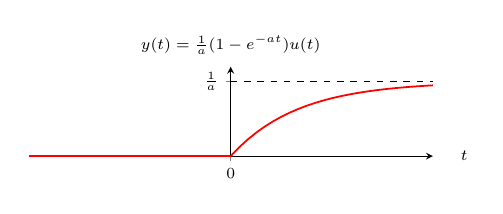
\begin{tikzpicture}[scale=0.8]
\begin{axis}[
	name=axis1,
       width=8cm,
       height=3cm,	
	axis y line=middle,
	axis x line=bottom,
	ymin=0,ymax=1.2,
	xmin=-3,xmax=3,	
	xlabel=$t$,
	ylabel= {$y(t) = \frac{1}{a}(1-e^{-at})u(t)$},	
	xtick={0},
	ytick={1},
	yticklabel={$\frac{1}{a}$},
	every axis x label/.style={at={(ticklabel* cs:1.05)},    anchor=west},
	every axis y label/.style={at={(ticklabel* cs:1.05)},    anchor=south},	
	clip=false,
]
	\addplot [thin, dashed] coordinates {(0,1) (3,1)};
	\addplot [thick, red] coordinates {(-3,0) (0,0)};
	\addplot [thick, red, domain=0:3] {1-exp(-x)}; 
\end{axis}

\end{tikzpicture} 
      \caption{Response}\label{fi:ct_conv_example26_sol}
    \end{figure}
    }
\end{frame}

\begin{frame}{}
    \textbf{ Example: } Consider the convolution of the following two signals:
    \begin{equation*}
        x(t) = \begin{cases}1,& 0 < t < T,\\ 0, & \text{otherwise}.\end{cases}
    \end{equation*}
    and
    \begin{equation*}
        h(t) = \begin{cases}t,& 0 < t < 2T,\\ 0, & \text{otherwise}.\end{cases}
    \end{equation*}


    \mode<beamer>
    {
        \begin{columns}
            \column{0.48\textwidth}
            \column{0.48\textwidth}
        \end{columns}
    }
\end{frame}

\begin{frame}<beamer>[plain,t]
    \mode<beamer>
    {
    \begin{figure}
      \centering
      \pgfplotsset{every axis/.append style={font=\scriptsize}}
\begin{tikzpicture}[scale=0.6]
\begin{axis}[
	name=axis1,
       width=8cm,
       height=3cm,	
	axis y line=middle,
	axis x line=bottom,
	ymin=0,ymax=1.2,
	xmin=-3,xmax=4,	
	xlabel=$\tau$,
	ylabel= $x(\tau)$,	
	xtick={0, 1},
	xticklabels={0, $T$},
	ytick={1},
	every axis x label/.style={at={(ticklabel* cs:1.05)},    anchor=west},
	every axis y label/.style={at={(ticklabel* cs:1.05)},    anchor=west},	
	clip=false,
]
	\addplot [thick, blue] coordinates {(-3,0) (0,0) (0,1) (1,1) (1,0) (4,0)};
\end{axis}
\pause
\begin{axis}[
	name=axis2,
	at={($(axis1.south east)+(0,-0.8cm)$)},anchor=north east,
       width=8cm,
       height=3cm,	
	axis y line=middle,
	axis x line=bottom,
	ymin=0,ymax=1.2,
	xmin=-3,xmax=4,	
	xlabel=$\tau$,
	ylabel= $h(t-\tau)$,	
	xtick={-2.5, -0.5, 0},
	xticklabels={$t-2T$, $t$, 0},
	ytick={1},
	yticklabels={$2T$},
	every axis x label/.style={at={(ticklabel* cs:1.05)},    anchor=west},
	every axis y label/.style={at={(ticklabel* cs:1.05)},    anchor=west},	
	clip=false,
]
	\addplot [dashed, blue] coordinates {(-3,0) (0,0) (0,1) (1,1) (1,0) (4,0)};
	\addplot [thick, red] coordinates {(-3,0) (-2.5,0) (-2.5,1) (-0.5, 0) (4,0)};

	\node at (axis cs:3,0.8) {$t<0$};	
\end{axis}
\pause
\begin{axis}[
	name=axis3,
	at={($(axis2.south east)+(0,-0.8cm)$)},anchor=north east,
       width=8cm,
       height=3cm,	
	axis y line=middle,
	axis x line=bottom,
	ymin=0,ymax=1.2,
	xmin=-3,xmax=4,	
	xlabel=$\tau$,
	ylabel= $h(t-\tau)$,	
	xtick={-1.5, 0.5, 0},
	xticklabels={$t-2T$, $t$, 0},
	ytick={1},
	yticklabels={$2T$},
	every axis x label/.style={at={(ticklabel* cs:1.05)},    anchor=west},
	every axis y label/.style={at={(ticklabel* cs:1.05)},    anchor=west},	
	clip=false,
]
	\addplot [dashed, blue] coordinates {(-3,0) (0,0) (0,1) (1,1) (1,0) (4,0)};
	\addplot [thick, red] coordinates {(-3,0) (-1.5,0) (-1.5,1) (0.5, 0) (4,0)};
	\node at (axis cs:3,0.8) {$0<t<T$};	
\end{axis}
\pause
\begin{axis}[
	name=axis4,
	at={($(axis3.south east)+(0,-0.8cm)$)},anchor=north east,
       width=8cm,
       height=3cm,	
	axis y line=middle,
	axis x line=bottom,
	ymin=0,ymax=1.2,
	xmin=-3,xmax=4,	
	xlabel=$\tau$,
	ylabel= $h(t-\tau)$,	
	xtick={-.5, 1.5},
	xticklabels={$t-2T$, $t$},
	ytick={1},
	yticklabels=\empty,
	every axis x label/.style={at={(ticklabel* cs:1.05)},    anchor=west},
	every axis y label/.style={at={(ticklabel* cs:1.05)},    anchor=west},	
	clip=false,
]
	\addplot [dashed, blue] coordinates {(-3,0) (0,0) (0,1) (1,1) (1,0) (4,0)};
	\addplot [thick, red] coordinates {(-3,0) (-.5,0) (-.5,1) (1.5, 0) (4,0)};
	\node at (axis cs:3,0.8) {$T<t<2T$};	
\end{axis}
\pause
\begin{axis}[
	name=axis5,
	at={($(axis4.south east)+(0,-0.8cm)$)},anchor=north east,
       width=8cm,
       height=3cm,	
	axis y line=middle,
	axis x line=bottom,
	ymin=0,ymax=1.2,
	xmin=-3,xmax=4,	
	xlabel=$\tau$,
	ylabel= $h(t-\tau)$,	
	xtick={.5, 2.5},
	xticklabels={$t-2T$, $t$},
	ytick={1},
	yticklabels={$2T$},
	every axis x label/.style={at={(ticklabel* cs:1.05)},    anchor=west},
	every axis y label/.style={at={(ticklabel* cs:1.05)},    anchor=west},	
	clip=false,
]
	\addplot [dashed, blue] coordinates {(-3,0) (0,0) (0,1) (1,1) (1,0) (4,0)};
	\addplot [thick, red] coordinates {(-3,0) (.5,0) (.5,1) (2.5, 0) (4,0)};
	\node at (axis cs:3,0.8) {$2T<t<3T$};	
\end{axis}
\pause
\begin{axis}[
	name=axis6,
	at={($(axis5.south east)+(0,-0.8cm)$)},anchor=north east,
       width=8cm,
       height=3cm,	
	axis y line=middle,
	axis x line=bottom,
	ymin=0,ymax=1.2,
	xmin=-3,xmax=4,	
	xlabel=$\tau$,
	ylabel= $h(t-\tau)$,	
	xtick={1.5, 3.5, 0},
	xticklabels={$t-2T$, $t$, 0},
	ytick={1},
	yticklabels={$2T$},
	every axis x label/.style={at={(ticklabel* cs:1.05)},    anchor=west},
	every axis y label/.style={at={(ticklabel* cs:1.05)},    anchor=west},	
	clip=false,
]
	\addplot [dashed, blue] coordinates {(-3,0) (0,0) (0,1) (1,1) (1,0) (4,0)};
	\addplot [thick, red] coordinates {(-3,0) (1.5,0) (1.5,1) (3.5, 0) (4,0)};
	\node at (axis cs:3,0.8) {$t>3T$};	
\end{axis}
\end{tikzpicture} 
      \caption{$x(\tau)$ and $h(t-\tau)$}\label{fi:ct_conv_example27}
    \end{figure}
    }
\end{frame}


\begin{frame}<beamer>[plain,t]
    \mode<beamer>
    {
    \begin{figure}
      \centering
      \pgfplotsset{every axis/.append style={font=\scriptsize}}
\begin{tikzpicture}[scale=1]


\begin{axis}[
	name=axis1,
       width=8cm,
       height=3cm,	
	axis y line=middle,
	axis x line=bottom,
	ymin=0,ymax=1.2,
	xmin=-3,xmax=4,	
	xlabel=$\tau$,
	ylabel= $x(\tau)h(t-\tau)$,	
	xtick={-2.5, -0.5, 0},
	xticklabels={$t-2T$, $t$, 0},
	ytick={0.25, 1},
	yticklabels={$t$, $2T$},
	every axis x label/.style={at={(ticklabel* cs:1.05)},    anchor=west},
	every axis y label/.style={at={(ticklabel* cs:1.05)},    anchor=west},	
	clip=false,
]
	\addplot [dashed, blue] coordinates {(-3,0) (0,0) (0,1) (1,1) (1,0) (4,0)};
	\addplot [thick, red] coordinates {(-3,0) (0,0) (0,0.25) (0.5, 0) (4,0)};

	\node at (axis cs:3,0.8) {$0<t<T$};	
\end{axis}

\begin{axis}[
	name=axis2,
	at={($(axis1.south east)+(0,-0.8cm)$)},anchor=north east,
       width=8cm,
       height=3cm,	
	axis y line=middle,
	axis x line=bottom,
	ymin=0,ymax=1.2,
	xmin=-3,xmax=4,	
	xlabel=$\tau$,
	ylabel= $x(\tau)h(t-\tau)$,	
	xtick={-1.5, 0.5, 0, 1},
	xticklabels={$t-2T$, $t$, 0, $T$},
	ytick={0.25,  0.75, 1},
	yticklabels={$t-T$, $t$, $2T$},
	every axis x label/.style={at={(ticklabel* cs:1.05)},    anchor=west},
	every axis y label/.style={at={(ticklabel* cs:1.05)},    anchor=west},	
	clip=false,
]
	\addplot [dashed, blue] coordinates {(-3,0) (0,0) (0,1) (1,1) (1,0) (4,0)};
	\addplot [thick, red] coordinates {(-3,0) (0,0) (0,0.75) (1,0.25) (1, 0) (4,0)};
	\node at (axis cs:3,0.8) {$T<t<2T$};	
\end{axis}

\begin{axis}[
	name=axis3,
	at={($(axis2.south east)+(0,-0.8cm)$)},anchor=north east,
       width=8cm,
       height=3cm,	
	axis y line=middle,
	axis x line=bottom,
	ymin=0,ymax=1.2,
	xmin=-3,xmax=4,	
	xlabel=$\tau$,
	ylabel= $x(\tau)h(t-\tau)$,	
	xtick={.5},
	xticklabels={$t-2T$},
	ytick={0.75, 1},
	yticklabels={$t-T$, $2T$},	
	every axis x label/.style={at={(ticklabel* cs:1.05)},    anchor=west},
	every axis y label/.style={at={(ticklabel* cs:1.05)},    anchor=west},	
	clip=false,
]
	\addplot [dashed, blue] coordinates {(-3,0) (0,0) (0,1) (1,1) (1,0) (4,0)};
	\addplot [thick, red] coordinates {(-3,0) (.5,0) (.5,1) (1, 0.75) (1,0) (4,0)};
	\node at (axis cs:3,0.8) {$2T<t<3T$};	
\end{axis}

\end{tikzpicture} 
      \caption{Product $x(\tau)h(t-\tau)$ for values of $t$ for which this product is not identically zero.}\label{fi:ct_conv_example27working}
    \end{figure}
    }
\end{frame}

\begin{frame}<beamer>[plain,t]
    \mode<beamer>
    {
    \begin{figure}
      \centering
      \pgfplotsset{every axis/.append style={font=\scriptsize}}
\begin{tikzpicture}[scale=1]


\begin{axis}[
	name=axis1,
       width=8cm,
       height=5cm,	
	axis y line=middle,
	axis x line=bottom,
	ymin=0,ymax=2,
	xmin=-3,xmax=4,	
	xlabel=$t$,
	ylabel= $y(t)$,	
	xtick={0, 1, 2, 3},
	xticklabels={0, $T$, $2T$, $3T$},
	ytick={0.25, 1},
	yticklabels=\empty,
	every axis x label/.style={at={(ticklabel* cs:1.05)},    anchor=west},
	every axis y label/.style={at={(ticklabel* cs:1.05)},    anchor=west},	
	clip=false,
]
	\addplot [dashed, blue] coordinates {(-3,0) (0,0) (0,1) (1,1) (1,0) (4,0)};
	\addplot [thick, red, domain=-3:0]  {0};
	\addplot [thick, red, domain=0:1]  {0.5*x*x};
	\addplot [thick, red, domain=1:2]  {x - 0.5};
	\addplot [thick, red, domain=2:3]  {-0.5*x*x + x +1.5};	
	\addplot [thick, red, domain=3:4]  {0};	
\end{axis}

\end{tikzpicture} 
      \caption{$y(t) = x(t)\ast h(t)$}\label{fi:ct_conv_example27sol}
    \end{figure}
    }
\end{frame}


\begin{frame}{}
    \textbf{ Example: } Find $y(t)$, the convolution of the following two signals:
    \begin{equation*}
        x(t) = e^{2t}u(-t),
    \end{equation*}
    and
    \begin{equation*}
        x(t) = u(t-3).
    \end{equation*}


    \mode<beamer>
    {
        \begin{columns}
            \column{0.48\textwidth}
            \column{0.48\textwidth}
        \end{columns}
    }
\end{frame}


\begin{frame}<beamer>[plain,t]
    \mode<beamer>
    {
    \begin{figure}
      \centering
      \pgfplotsset{every axis/.append style={font=\scriptsize}}
\begin{tikzpicture}[scale=0.8]


\begin{axis}[
	name=axis1,
       width=8cm,
       height=4cm,	
	axis y line=middle,
	axis x line=bottom,
	ymin=0,ymax=1.5,
	xmin=-4,xmax=4,	
	xlabel=$\tau$,
	ylabel={$x(\tau) = e^{2\tau}u(-\tau)$},	
	xtick={0},
	xticklabels={0},
	ytick={1},
	yticklabels={1},
	every axis x label/.style={at={(ticklabel* cs:1.05)},    anchor=west},
	every axis y label/.style={at={(ticklabel* cs:1.05)},    anchor=west},	
	clip=false,
]
	\addplot [thick, red, domain=-3:0]  {exp(2*x)};
\end{axis}

\pause
\begin{axis}[
	name=axis2,
	at={($(axis1.south east)+(0,-0.8cm)$)},anchor=north east,
       width=8cm,
       height=4cm,	
	axis y line=middle,
	axis x line=bottom,
	ymin=0,ymax=1.5,
	xmin=-4,xmax=4,	
	xlabel=$\tau$,
	ylabel={$h(t-\tau)$},	
	xtick={-3, 0},
	xticklabels={$t-3$, 0},
	ytick={1},
	yticklabels={1},
	every axis x label/.style={at={(ticklabel* cs:1.05)},    anchor=west},
	every axis y label/.style={at={(ticklabel* cs:1.05)},    anchor=west},	
	clip=false,
]
	\addplot [thick, red, domain=-3:0]  coordinates {(-4, 1) (-3,1) (-3, 0) (4,0)};
\end{axis}

\pause
\begin{axis}[
	name=axis3,
	at={($(axis2.south east)+(0,-0.8cm)$)},anchor=north east,
       width=8cm,
       height=4cm,	
	axis y line=middle,
	axis x line=bottom,
	ymin=0,ymax=1.5,
	xmin=-4,xmax=4,	
	xlabel=$t$,
	ylabel={$y(t)$},	
	xtick={3, 0},
	xticklabels={$3$, 0},
	ytick={0.5, 1},
	yticklabels={$\frac{1}{2}$, 1},
	every axis x label/.style={at={(ticklabel* cs:1.05)},    anchor=west},
	every axis y label/.style={at={(ticklabel* cs:1.05)},    anchor=west},	
	clip=false,
]
	\addplot [thick, red, domain=-3:3]  {0.5*exp(2*(x-3))};
	\addplot [thick, red, domain=-3:0]  coordinates {(3, 0.5) (4, 0.5)};	
\end{axis}

\end{tikzpicture} 
      \caption{Convolution considered in the example.}\label{fi:ct_conv_example28}
    \end{figure}
    }
\end{frame}


\begin{frame}
    When $t-3 \leq 0$, the product of $x(\tau)$ and $h(t-\tau)$ is nonzero for $-\infty < \tau < t-3$, and the convolving integral becomes
    \begin{equation*}
        y(t) = \int_{-\infty}^{t-3}e^{2\tau}d\tau = \frac{1}{2}e^{2(t-3)}.
    \end{equation*}
    F0r $t-3 \geq 0$, the product of $x(\tau)h(t-\tau)$ is nonzero for $-\infty < \tau < 0$, and the convolving integral becomes
    \begin{equation*}
        y(t) = \int_{-\infty}^{0}e^{2\tau}d\tau = \frac{1}{2}.
    \end{equation*}
\end{frame}



\section{Properties of Linear Time-Invariant Systems}


\begin{frame}{Recapitulation}
    \begin{enumerate}
        \item In discrete time the representation takes the form of the convolution sum, while its continuous-time counterpart is the convolution integral:
            \begin{align*}
                y[n] &= \sum_{k=-\infty}^{\infty}x[k]h[n-k] = x[n]\ast h[n]\\
                y(t) &= \int_{-\infty}^{\infty}x(\tau)h(t-\tau)d\tau = x(t)\ast h(t)\\
            \end{align*}
        \item Characteristics of an LTI system are completely determined by its impulse response.
    \end{enumerate}

\end{frame}



\begin{frame}{The Commutative Property}
    DT
    \begin{equation*}
        x[n]\ast h[n] = h[n] \ast x[n] = \sum_{k=-\infty}^{\infty}h[k]x[n-k].
    \end{equation*}
    CT
    \begin{equation*}
        x(t)\ast h(t) = h(t) \ast x(t) = \int_{-\infty}^{\infty}h(\tau)x(t-\tau)d\tau.
    \end{equation*}

    Verify the commutative property for DT.
    \pause
    \mode<beamer>
    {
        \begin{columns}
            \column{0.48\textwidth}
                \begin{equation*}
                    x[n]\ast h[n] = \sum_{k=-\infty}^{\infty}x[k]h[n-k].
                \end{equation*}
                Substituting $r = n-k$, or equivalently $k = n-r$
                \pause
                \begin{equation*}
                    x[n]\ast h[n] = \sum_{k=-\infty}^{\infty}x[n-r]h[r] = h[n]\ast x[n].
                \end{equation*}
            \column{0.48\textwidth}
        \end{columns}
    }
\end{frame}

\begin{frame}{The Distributive Property}
Convolution distributes over addition.\par
    DT
    \begin{equation*}
        x[n]\ast (h_1[n] + h_2[n]) = x[n]\ast h_1[n] + x[n]\ast  h_2[n].
    \end{equation*}
    CT
    \begin{equation*}
        x(t)\ast (h_1(t) + h_2(t)) = x(t)\ast h_1(t) + x(t)\ast  h_2(t).
    \end{equation*}


    \mode<beamer>
    {
        \begin{figure}
          \centering
          \tikzstyle{int}=[draw, fill=pink!60, minimum size=2em]
\tikzstyle{init} = [pin edge={to-,thin,black}]

\begin{tikzpicture}[node distance=2.5cm,auto,>=latex']

	\begin{scope}[node distance=1cm and 0.5cm,auto,>=latex']
		\node (a) at (0,0) {$x(t)$};
		\node (b) [right of=a, coordinate] {};
		\node (c) [int, above right = of b] {$h_1(t)$};
		\node (d) [int, below right = of b] {$h_2(t)$};		
		\draw (a) -- (b);
		\draw[-latex] (b) |- (c);
		\draw[-latex] (b) |- (d);	
		\node (e) [right = of b, xshift=2cm, circle, draw, fill=white] {$+$};
		\draw[] (c) -| node[near start, above] {$y_1(t)$} (e.north);		
		\draw[] (d) -|  node[near start, below] {$y_2(t)$} (e);	
		\node (f) [right of=e, xshift=0.5cm] {$y(t)$};	
		\draw[-latex] (e.east) |- (f);	
	\end{scope}
	
	\begin{scope}[yshift=-3cm,
		start chain,
		node distance=5mm,
		every node/.style={int, draw,on chain,join,inner sep=2mm},
		every join/.style={->}
		]
		\node[draw=none, fill=none]  {$x(t)$};	
		\node { $h_1(t) + h_2$};
		\node[draw=none, fill=none]   {$y(t)$};
	\end{scope}
	
	
\end{tikzpicture} 
          \caption{Distributive property.}\label{fi:distributive_property}
        \end{figure}
    }
\end{frame}



\begin{frame}{The Associative Property}
    DT
    \begin{equation*}
        x[n]\ast (h_1[n] \ast h_2[n]) = (x[n]\ast h_1[n]) \ast h_2[n].
    \end{equation*}
    CT
    \begin{equation*}
        x(t)\ast (h_1(t) \ast h_2(t)) = (x(t)\ast h_1(t)) \ast h_2(t).
    \end{equation*}
    As a consequence,
    \begin{equation*}
        y[n] = x[n]\ast h_1[n] \ast h_2[n]
    \end{equation*}
    and
    \begin{equation*}
        y(t) = x(t)\ast h_1(t) \ast h_2(t) .
    \end{equation*}
    are unambiguous.\par
    Using the commutative property together with the associative property we can see that the order in which they are cascaded does not matter as far as the overall system impulse response is concerned.

% TODO include Figure 225
    \mode<beamer>
    {
        \begin{columns}
            \column{0.48\textwidth}
            \column{0.48\textwidth}
        \end{columns}
    }
\end{frame}


\begin{frame}[plain]
    \mode<beamer>
    {
        \begin{figure}
          \centering
          \tikzstyle{int}=[draw, fill=pink!60, minimum size=2em]
\tikzstyle{init} = [pin edge={to-,thin,black}]

\begin{tikzpicture}[node distance=2.5cm,auto,>=latex']

	\begin{scope}[yshift=0cm,
		start chain,
		node distance=5mm,
		every node/.style={int, draw,on chain,join,inner sep=2mm},
		every join/.style={->}
		]
		\node[draw=none, fill=none]  {$x[n]$};	
		\node { $h_1[n]$};
		\node { $h_2[n]$};
		\node[draw=none, fill=none]   {$y[n]$};
	\end{scope}
	\pause
	
	\begin{scope}[yshift=-2cm,
		start chain,
		node distance=5mm,
		every node/.style={int, draw,on chain,join,inner sep=2mm},
		every join/.style={->}
		]
		\node[draw=none, fill=none]  {$x[n]$};	
		\node { $h[n] = h_1[n] \ast h_2[n]$};
		\node[draw=none, fill=none]   {$y[n]$};
	\end{scope}
	\pause
	\begin{scope}[yshift=-4cm,
		start chain,
		node distance=5mm,
		every node/.style={int, draw,on chain,join,inner sep=2mm},
		every join/.style={->}
		]
		\node[draw=none, fill=none]  {$x[n]$};	
		\node { $h[n] = h_2[n] \ast h_1[n]$};
		\node[draw=none, fill=none]   {$y[n]$};
	\end{scope}	
	\pause
	\begin{scope}[yshift=-6cm,
		start chain,
		node distance=5mm,
		every node/.style={int, draw,on chain,join,inner sep=2mm},
		every join/.style={->}
		]
		\node[draw=none, fill=none]  {$x[n]$};	
		\node { $h_2[n]$};
		\node { $h_1[n]$};
		\node[draw=none, fill=none]   {$y[n]$};
	\end{scope}
		
	
	
\end{tikzpicture} 
          \caption{Associative property.}\label{fi:associative_property}
        \end{figure}
    }
\end{frame}


\begin{frame}{LTI Systems with and without Memory}
    \begin{enumerate}
        \item A system is memoryless if its output at any time depends only on the value of the input at that same time.
        \item The only way that this can be true for a discrete-time LTI system is if $h[n] = 0$ for $n \neq 0$.
        \item In this case the impulse response has the form
        \begin{equation*}
            h[n] = K\delta[n],
        \end{equation*}
        where $K = h[0]$ is a constant.
        \item The convolution sum reduces to the relation
        \begin{equation*}
            y[n] = Kx[n]
        \end{equation*}
        \item If a discrete-time LTI system has an impulse response $h[n]$ that is not identically zero for $n \neq 0$, then the system has memory.
        \item For CT:
            \begin{align*}
                h(t) &= K\delta(t).\\
                y(t) &= Kx(t).\\
            \end{align*}
    \end{enumerate}

\end{frame}





\begin{frame}{lnvertibility of LTI Systems}
    \begin{enumerate}
        \item An LTI system is invertible only if an inverse system exists that, when connected in series with the original system, produces an output equal to the input to the first system.
    \end{enumerate}

    \mode<beamer>
    {
    \begin{figure}
      \centering
      \tikzstyle{int}=[draw, fill=pink!60, minimum size=2em]
\tikzstyle{init} = [pin edge={to-,thin,black}]

\begin{tikzpicture}[node distance=2.5cm,auto,>=latex']

		\node (a) at (0,0) {$x(t)$};
	\node (b)  [int, right of=a, node distance=2cm] {$h(t)$};
	\node (c)  [int, right of=b, node distance=2cm] {$h_1(t)$};
	\node (d)  [right of=c, node distance=2cm] {$w(t) = x(t)$};	
	\path[->] (a) edge (b);
	\path[->] (b) edge node {$y(t)$} (c);
	\draw[->] (c) edge (d) ;
	
	\begin{scope}[yshift=-2cm,
		start chain,
		node distance=5mm, 
		every node/.style={int, draw,on chain,join,inner sep=2mm}, 
		every join/.style={->}
		]
		\node[draw=none, fill=none]  {$x(t)$};	
		\node {Identity system $\delta(t)$};
		\node[draw=none, fill=none]   {$x(t)$};
	\end{scope}
	
	
\end{tikzpicture}


      \caption{Inverse of a CT LTI system.}\label{fi:lti_inverse}
    \end{figure}
    }
\end{frame}


\begin{frame}{}
    \textbf{ Example}\par
    Consider the following relationship of a pure time shift:
    \begin{equation*}
        y(t) = x(t-t_0)
    \end{equation*}
    Is the corresponding system memoryless? What is the inverse system of the system? \pause

    \mode<beamer>
    {
        Delay if $t_0 > 0$, and advance if $t_0 < 0$. E.g., if $t_0 > 0$ then the output at time $t$ equals the input at the earlier time $t-t_0$. If $t_0 = 0$, the system is the identity system  and that is memoryless. For any other value of $t_0$, the system has memory. \par
        \pause
        Setting the input equal to $\delta(t)$, the impulse response can be obtained:
        \begin{equation*}
            h(t) = \delta(t-t_0).
        \end{equation*}
        Therefore,
        \begin{equation*}
            x(t-t_0) = x(t)\ast \delta(t-t_0).
        \end{equation*}
        That is, the convolution of a signal with a shifted impulse simply shifts the signal. To recover the input from the output, i.e., to invert the system, all that is required is to shift the output back.
        \begin{equation*}
            h_1(t) = \delta(t+t_0).
        \end{equation*}
        Then
        \begin{equation*}
            h(t)\ast h_1(t) = \delta(t-t_0) \ast \delta(t+t_0) = \delta(t).
        \end{equation*}
    }
\end{frame}

\begin{frame}{}
    \textbf{ Example}\par
    Consider the LTI system with impulse response
    \begin{equation*}
        h[n] = u[n].
    \end{equation*}
    Determine $y[n]$. Find the inverse system.
    \mode<beamer>
    {
        %TODO: Type answer from example 2.12
    }
\end{frame}


\begin{frame}{Causality for LTI Systems}

    \begin{enumerate}
        \item The output of a causal system depends only on the present and past values of the input to the system.
        \item For a DT LTI system, $y[n]$ must not depend on $x[k]$ for $k > n$.
        \item For this to be true, all of the coefficients $h[n- k]$ that multiply values of $x[k]$ for $k > n$ must be zero.
        \item This then requires that the impulse response of a causal discrete-time LTI system satisfy the condition
            \begin{equation*}
                h[n] = 0\quad \text{for } n < 0.
            \end{equation*}
        \item The impulse response of a causal LTI system must be zero before the impulse occurs, which is consistent with the intuitive concept of causality.
        \item More generally, causality for a linear system is equivalent to the condition of initial rest; i.e., if the input to a causal system is 0 up to some point in time, then the output must also be 0 up to that time.
        \item The equivalence of causality and the condition of initial rest applies only to linear systems.
    \end{enumerate}
\end{frame}

\begin{frame}{Causality for LTI Systems}

    \begin{enumerate}
        \item A continuous-time LTI system is causal if
            \begin{equation*}
                h(t) = 0\quad \text{for } t < 0.
            \end{equation*}
        \item Causality of an LTI system is equivalent to its impulse response being a causal signal.
    \end{enumerate}
\end{frame}

\begin{frame}{Stability for LTI Systems}
A system is stable if every bounded input produces a bounded output. Consider an input $x[n]$ that is bounded in magnitude:
    \begin{align*}
        |x[n]| &< B \quad \text{for all } n.\\
      |y[n]| &= \left| \sum_{k=-\infty}^{\infty}h[k]x[n-k]\right| \\
      |y[n]| &\leq  \sum_{k=-\infty}^{\infty}|h[k]||x[n-k]|\\
      |y[n]| &\leq  B\sum_{k=-\infty}^{\infty}|h[k]|\quad \text{for all } n\\
      \sum_{k=-\infty}^{\infty}|h[k]| &< \infty.\\
    \end{align*}
    If the impulse response is absolutely summable, then $y[n]$ is bounded in magnitude, and hence, the system is stable.

\end{frame}

\begin{frame}{Stability for LTI Systems}
    In CT a system is stable if the impulse response is \alert{absolutely integrable}.
    \begin{equation*}
        \int_{-\infty}^{\infty}|h(\tau)|d\tau < \infty.
    \end{equation*}
\end{frame}




\begin{frame}{}
    \textbf{ Examples}\par
    Determine whether the following systems are stable:
    \begin{enumerate}
        \item Pure time shift in DT.
        \item Pure time shift in CT.
        \item Accumulator in DT.
        \item CT counterpart of the accumulator.
    \end{enumerate}

    \mode<beamer>
    {
        \begin{columns}
            \column{0.48\textwidth}
            Pure time shift in DT:\par
            \begin{equation*}
                \sum_{n=-\infty}^{\infty}|h[n]| = \sum_{n=-\infty}^{\infty}|\delta[n-n_0]| = 1
            \end{equation*}
            \pause
            Ans:\textcolor{YellowGreen}{stable.}\par
            \pause
            Pure time shift in CT:\par
            \begin{equation*}
                \int_{-\infty}^{\infty}|h(\tau)d\tau| = \int_{-\infty}^{\infty}|\delta(\tau- t_0)d\tau| = 1
            \end{equation*}
            \pause
            Ans: \textcolor{YellowGreen}{stable.}\par
            Accumulator in DT: $h[n] = u[n]$\par
            \begin{equation*}
                \sum_{n=-\infty}^{\infty}|u[n]| = \sum_{n=0}^{\infty}|u[n]| = \infty
            \end{equation*}
            \pause
            Ans: \textcolor{Tomato}{unstable.}
            \pause
            \column{0.48\textwidth}

            CT counterpart of the accumulator:
            \begin{equation*}
                y(t) = \int_{-\infty}^{t}x(\tau)d\tau
            \end{equation*}
            The impulse response of the integrator can be found by letting $x(t) = \delta(t)$:
            \begin{equation*}
                h(t) = \int_{-\infty}^{t}\delta(\tau)d\tau = u(t).
            \end{equation*}
            \begin{equation*}
                \int_{-\infty}^{\infty}|u(\tau)d\tau| = \int_{0}^{\infty}d\tau| = \infty
            \end{equation*}
            \pause
            Ans: \textcolor{Tomato}{unstable.}
        \end{columns}
    }
\end{frame}




\begin{frame}{The Unit Step Response of an LTI System}
    There is another signal that is also used in describing the behavior of LTI systems: the unit step response, $s[n]$ or $s(t)$, corresponding to the output when $x[n] =
u[n]$ or $x(t) = u(t)$.


    %\mode<beamer>
    {
        \begin{columns}
            \column{0.48\textwidth}
                \mode<beamer>
                {
                    \begin{figure}
                      \centering
                      \tikzstyle{int}=[draw, fill=pink!60, minimum size=2em]
\tikzstyle{init} = [pin edge={to-,thin,black}]

\begin{tikzpicture}[node distance=2.5cm,auto,>=latex']
	
	\begin{scope}[yshift=-2cm,
		start chain,
		node distance=5mm,
		every node/.style={int, draw,on chain,join,inner sep=2mm},
		every join/.style={->}
		]
		\node[draw=none, fill=none]  {$u[n]$};	
		\node { $h[n]$};
		\node[draw=none, fill=none]   {$s[n]$};
	\end{scope}
	
	
\end{tikzpicture} 
                      \caption{Unit step response.}\label{fi:step_resp}
                    \end{figure}
                }

                \begin{equation*}
                    s[n] = u[n] \ast h[n]
                \end{equation*}
                Commutative property:
                \begin{equation*}
                    s[n] = h[n] \ast u[n]
                \end{equation*}
                $s[n]$ can be viewed as the response to the input $h[n]$ of a discrete-time LTI system with unit impulse response $u[n]$.

            \column{0.48\textwidth}
                \mode<beamer>
                {
                    \begin{figure}
                      \centering
                      \tikzstyle{int}=[draw, fill=pink!60, minimum size=2em]
\tikzstyle{init} = [pin edge={to-,thin,black}]

\begin{tikzpicture}[node distance=2.5cm,auto,>=latex']
	
	\begin{scope}[yshift=-2cm,
		start chain,
		node distance=5mm,
		every node/.style={int, draw,on chain,join,inner sep=2mm},
		every join/.style={->}
		]
		\node[draw=none, fill=none]  {$h[n]$};	
		\node { $u[n]$};
		\node[draw=none, fill=none]   {$s[n]$};
	\end{scope}
	
	
\end{tikzpicture}
                      \caption{Unit step response.}\label{fi:step_resp_switched}
                    \end{figure}
                }
                $u[n]$ is the unit impulse response of the accumulator. Therefore,
                \begin{equation*}
                    s[n] = \sum_{k=-\infty}^{\infty}h[k]
                \end{equation*}
                $h[n]$ can be recovered from $s[n]$ using the relation
                \begin{equation*}
                    h[n] = s[n] - s[n - 1].
                \end{equation*}


        \end{columns}
    }
\end{frame}

\begin{frame}{}
    \textcolor{Tomato}{That is, the step response of a discrete-time LTI system is the running sum of its impulse response. Conversely, the impulse response of a discrete-time LTI system is the first difference of its step response.}\par
    Similarly, in CT, the step response of an LTI system with impulse response $h(t)$ is given by $s(t) = u(t) \ast h(t)$, which also equals the response of an integrator
    [with impulse response $u(t)$] to the input $h(t)$. That is, the unit step response of a continuous-time LTI system is the running integral of its impulse response, or
    \mode<beamer>
    {
        \begin{equation*}
            s(t) = \int_{-\infty}^{t}h(\tau)d\tau
        \end{equation*}
    the unit impulse response is the first derivative of the unit step response, or
        \begin{equation*}
            h(t) = \frac{ds(t)}{d(t)} = s^\prime(t).
        \end{equation*}
    }
\end{frame}




\begin{frame}{Zero-Input Response}
    For a linear system (time-invariant or not), if we put nothing into it, we get nothing out of it.
    \begin{align*}
        x(t)  &= 0 \quad \text{for all } t, \quad \text{then}\\
        y(t)  &= 0 \quad \text{for all } t,\\
        x[n]  &= 0 \quad \text{for all } n, \quad \text{then}\\
        y[n]  &= 0 \quad \text{for all } n,
    \end{align*}
    ``Proof'': If the system is linear and
    \begin{equation*}
        x(t) \rightarrow y(t), \quad \text{then if we scale}
    \end{equation*} \pause
    \begin{equation*}
        ax(t) \rightarrow ay(t).
    \end{equation*}
    Select the sale factor $a=0$.\par
    Not all systems are like this, e.g., even if a battery is not connected to anything, the output is 1.5 V.
\end{frame}

\begin{frame}{Implications for Causality}
    The system cannot anticipate the input.\par
    I.e.,
    If
    \begin{equation*}
        x_1(t) = x_2(t), \quad \text{for } t < t_0,
    \end{equation*}
    then
    \begin{equation*}
        y_1(t) = y_2(t), \quad \text{for } t < t_0,
    \end{equation*}
    Same for DT.
\end{frame}

\begin{frame}{Implications for Causality for a Linear System}
    For linear systems, if
    \mode<beamer>
    {
    \begin{equation*}
        x(t) =0, \quad \text{for } t < t_0,
    \end{equation*}
    then
    \begin{equation*}
        y(t) =0, \quad \text{for } t < t_0,
    \end{equation*}
    }
    \mode<handout>
    {
        \vspace{1.5in}
    }
    Initial rest: The system does not respond until an input is given.\par For a linear system to be causal it must have the property of initial rest.\par
    Why?\pause~ For linear systems zero in $\rightarrow$ zero out.  \par

\end{frame}

\begin{frame}{Causality for Linear Time Invariant Systems}    For LTI systems,
    \begin{equation*}
        \text{Causality} \Leftrightarrow \begin{split}h(t) = 0, \quad  t <0\\  h[n] = 0, \quad  n <0\\      \end{split}
    \end{equation*}
    ``Proof":
    $\Rightarrow$:  Why does causality imply the above? \pause~Ans:
    \mode<beamer>
    {
    \begin{align*}
      \delta(t) &=  0, t<0\\
      \delta[n] &=  0, n<0\\
    \end{align*}
    }
    \mode<handout>
    {
        \vspace{.5in}
    }
    \pause
    $\Leftarrow$:Why does $h(t) = 0, \quad  t <0$ ($h[n] = 0, \quad  n <0$, imply the system is causal?\pause~Ans:
    \mode<beamer>
    {
    \begin{equation*}
        \begin{split}
            y[n] = \sum_{k=-\infty}^{\infty}x[k]h[n-k] \quad & y(t) = \int_{-\infty}^{\infty}x(\tau)h(t-\tau)\\ \pause
            y[n] = \sum_{k=-\infty}^{n}x[k]h[n-k] \quad & y(t) = \int_{-\infty}^{t}x(\tau)h(t-\tau)
        \end{split}
    \end{equation*}
    Only values of $x[n]$ up until $n$ are used to compute  $y[n]$ (causal). Similar in CT case.
    }
\end{frame}

\begin{frame}{Example: Accumulator}

    \begin{equation*}
        y[n] = \sum_{k=-\infty}^{n}x[k]
    \end{equation*}
    The accumulator is an LTI system. Also, we saw that its impulse response is
    \begin{equation*}
        h[n] = u[n].
    \end{equation*}

    \begin{columns}
        \column{0.48\textwidth}

            \begin{enumerate}
              \item Does the accumulator have memory?
              \item Is the accumulator causal?
              \item Is accumulator stable in the BIBO sense?
              \item If invertible, what is the inverse?
            \end{enumerate}

            \pause
            \mode<beamer>
            {
            \begin{enumerate}[<+->]
                \item $h[n] \neq k\delta[n].$: has memory
                \item $h[n] = 0, \quad n < 0$: is causal
                \item $\sum_{k=-\infty}^{n}|h[n]| = \infty$ : not stable
            \end{enumerate}
            }
        \pause
        \column{0.48\textwidth}
            \mode<beamer>
            {
            Inverse $h[n] = u[n]$, $h^{-1}[n] =?$:\par
            Accumulator can be expressed as a \alert{recursive difference equation} as
            \begin{equation*}
                \begin{split}
                    y[n] &= \sum_{k=-\infty}^{n-1}x[k] + x[n]\\ \pause
                    &= y[n-1] + x[n].
                \end{split}
            \end{equation*}
            }

    \end{columns}

\end{frame}

\begin{frame}[plain]


    \mode<beamer>
    {
        \begin{columns}
            \column{0.48\textwidth}
                \begin{figure}
                  \centering
                  \tikzstyle{int}=[draw, fill=pink!60, minimum size=2em]
\tikzstyle{init} = [pin edge={to-,thin,black}]

\begin{tikzpicture}[node distance=3cm,auto,>=latex']
	
	\begin{scope}[yshift=-2cm,
		start chain,
		node distance=10mm,
		every node/.style={int, draw,join,inner sep=2mm},
		every join/.style={->}
		]
		\node (a) [draw=none, on chain, fill=none]  {$\delta[n]$};	
		\node (b) [on chain] {$h[n]$};
		\node (c) [on chain] {$h^{-1}[n]$};
		\node(d) [draw=none, on chain, fill=none]   {$\delta[n]$};
		\draw[->] (b) -- node[midway, above, fill=none, draw=none]   {$u[n]$}  node[midway, below, fill=none, draw=none]  {$x_2[n]$} (c);
		\draw[->] (c)-- node[midway, below, fill=none, draw=none]   {$y_2[n]$}  (d);
	\end{scope}
	
	
\end{tikzpicture}


                  \caption{}\label{fi:accumulator_inverse}
                \end{figure}
                We know that
                \begin{equation*}
                    u[n] - u[n-1] = \delta[n].
                \end{equation*}
                So
                \begin{equation*}
                    x_2[n] - x_2[n-1] = y_2[n].
                \end{equation*}
                \begin{equation*}
                    \delta[n] - \delta[n-1] = h^{-1}[n].
                \end{equation*}
            \column{0.48\textwidth}
            Inverse of the accumulator:
            \begin{enumerate}
              \item Does it have memory? Yes.
              \item Is the sysetm causal? Yes.
              \item Is the system stable in the BIBO sense? Yes.
            \end{enumerate}

        \end{columns}
    }
\end{frame}


\begin{frame}{Example}
    \begin{equation*}
        y[n] - ay[n-1] = x[n]
    \end{equation*}
    under the assumption of initial rest $\Rightarrow$ LTI.
    Memory? Causal? Stable?
    \pause
    \mode<beamer>
    {
        \begin{align*}
          x[n] &= \delta[n] \\
          h[n] &= a^nu[n] \quad (\text{Why?})\\
        \end{align*}
        \pause
            \begin{enumerate}
              \item Memory? Yes.
              \item Causal? Yes.
              \item Stable? If $|a|<1$, yes.
            \end{enumerate}
    }
\end{frame}

\begin{frame}{Example}
    \begin{equation*}
        \frac{dy(t)}{dt} +2y(t) = x(t)
    \end{equation*}
    under the assumption of initial rest $\Rightarrow$ LTI.
    Memory? Causal? Stable?
    \pause
    \mode<beamer>
    {
        \begin{align*}
          h(t) &= e^{-2t}u(t) \quad (\text{Why?})\\
        \end{align*}
        \pause
            \begin{enumerate}
              \item Memory? Yes.
              \item Causal? Yes.
              \item Stable? Yes.
            \end{enumerate}
    }
\end{frame}


\begin{frame}{Impulses}


    %\mode<beamer>
    {
        \begin{columns}
            \column{0.48\textwidth}
                \begin{figure}
                    \centering
                    \begin{tikzpicture}[start chain, system/.style={draw, fill=pink!60, minimum size=2em, align=center}]
	\node (a) [on chain, text width=2em] {$x(t)$\\ $x[n]$};
	\node (b) [system, on chain, text width=2em] {$h(t)$ \\ $h[n]$};
	\node (c) [on chain, text width=2em] {$y(t)$ \\ $y[n]$};	
	\draw[-latex] (a) -- (b);
	\draw[-latex] (b) -- (c);
\end{tikzpicture}
                    \caption{}\label{fi:sys_for_operational_def_1}
                \end{figure}

                \begin{figure}
                    \centering
                    \begin{tikzpicture}[start chain, system/.style={draw, fill=pink!60, minimum size=2em, align=center}]
	\node (a) [on chain, text width=2em] {$x(t)$\\ $x[n]$};
	\node (b) [system, on chain, text width=2em] {$I$};
	\node (c) [on chain, text width=2em] {$x(t)$ \\ $x[n]$};	
	\draw[-latex] (a) -- (b);
	\draw[-latex] (b) -- (c);
\end{tikzpicture}
                    \caption{}\label{fi:sys_for_operational_def_2}
                \end{figure}
                \pause
                \mode<beamer>
                {
                \begin{align*}
                  h(t) &= \delta(t) \\
                  h[n] &= \delta[n]
                \end{align*}
                }
                \mode<handout>
                {
                    \vspace{0.5in}
                }
                \pause
            \column{0.48\textwidth}
                \begin{figure}
                    \centering
                    \begin{tikzpicture}[start chain, system/.style={draw, fill=pink!60, minimum size=2em, align=center}]
	\node (a) [on chain, text width=2em] {$x(t)$\\ $x[n]$};
	\node (b) [system, on chain, text width=2em] {$I$};
	\node (c) [system, on chain, text width=2em] {$I$};	
	\node (d) [on chain, text width=2em] {$x(t)$ \\ $x[n]$};	
	\draw[-latex] (a) -- (b);
	\draw[-latex] (b) -- node[midway, above] {$x(t)$} node[midway, below] {$x[n]$} (c);
	\draw[-latex] (c) -- (d);	
\end{tikzpicture}
                    \caption{}\label{fi:sys_for_operational_def_3}
                \end{figure}
                \pause
                \mode<beamer>
                {
                \begin{align*}
                   \delta(t)\ast  \delta(t) &= \delta(t) \\
                    \delta[n] \ast \delta[n] &= \delta[n]
                \end{align*}
                }
                \mode<handout>
                {
                    \vspace{0.5in}
                }
                \pause
                \begin{figure}
                    \centering
                    \begin{tikzpicture}
	\begin{axis}
	[
		name=axis1,
	       width=4cm,
	       height=3cm,	
		axis y line=middle,
		axis x line=bottom,
		ymin=0,ymax=1.5,
		xmin=-4,xmax=4,	
		xlabel=$n$,
		ylabel={$\delta[n]$},	
		xtick={0},
		xticklabels={0},
		ytick={1},
		yticklabels={1},
		every axis x label/.style={at={(ticklabel* cs:1.05)},    anchor=west},
		every axis y label/.style={at={(ticklabel* cs:1.05)},    anchor=west},	
		clip=false,
	]
	\addplot[ycomb,  red, very thick, mark=*,] coordinates {(0,1)};
	\node at (axis cs:4, 0.5) [anchor=west] {No problem in DT.};
	
	\end{axis}
\end{tikzpicture}
                    \caption{}\label{fi:sys_for_operational_def_4}
                \end{figure}
        \end{columns}
    }
\end{frame}

\begin{frame}{}


    \mode<beamer>
    {
        \begin{columns}
            \column{0.48\textwidth}
                \begin{figure}
                    \centering
                    \begin{tikzpicture}
	\begin{axis}
	[
		name=axis1,
	       width=6cm,
	       height=3cm,	
		axis y line=middle,
		axis x line=bottom,
		ymin=0,ymax=1.5,
		xmin=-3,xmax=3,	
		xlabel=$t$,
		ylabel={$\delta_\Delta(t)$},	
		xtick={0, 1},
		xticklabels={0, $\Delta$},
		ytick={1},
		yticklabels={$\frac{1}{\Delta}$},
		every axis x label/.style={at={(ticklabel* cs:1.05)},    anchor=west},
		every axis y label/.style={at={(ticklabel* cs:1.05)},    anchor=west},	
		clip=false,
	]
	\addplot[red, very thick] coordinates {(0,0) (0,1) (1,1) (1,0)};
	
	\node at (axis cs:4, 0.5) [anchor=west] {$\delta(t) = \lim_{\Delta \rightarrow 0} \delta_\Delta(t)$};
	
	\end{axis}
	
	\begin{axis}
	[
		name=axis2,
		at={($(axis1.south east)+(0,-1.1cm)$)},anchor=north east,		
	       width=6cm,
	       height=3cm,	
		axis y line=middle,
		axis x line=bottom,
		ymin=0,ymax=1.5,
		xmin=-3,xmax=3,	
		xlabel=$t$,
		ylabel={$r_\Delta(t)$},	
		xtick={0, 1, 2},
		xticklabels={0, $\Delta$,  $2\Delta$},
		ytick={1},
		yticklabels={$\frac{1}{\Delta}$},
		every axis x label/.style={at={(ticklabel* cs:1.05)},    anchor=west},
		every axis y label/.style={at={(ticklabel* cs:1.05)},    anchor=west},	
		clip=false,
	]
	\addplot[red, very thick] coordinates {(0,0) (1,1) (2,0)};
	
	\node at (axis cs:4, 0.5) [anchor=west, text width=4cm] {$r_\Delta(t) = \delta_\Delta(t) \ast \delta_\Delta(t)$\\ $\delta(t) = \lim_{\Delta \rightarrow 0} r_\Delta(t)?$};
	
	\end{axis}	
\end{tikzpicture}
                    \caption{}\label{fi:sys_for_operational_def_5}
                \end{figure}
            \column{0.48\textwidth}
                \begin{figure}
                    \centering
                    \begin{tikzpicture}[start chain, system/.style={draw, fill=pink!60, minimum size=2em, align=center}]
	\node (a) [on chain, text width=2em] {$\delta(t)$\\ $x(t)$};
	\node (b) [system, on chain, text width=2em] {$\dfrac{d}{dt}$};
	\node (c) [on chain, text width=2em] {$?$ \\ $\dfrac{dx(t)}{dt}$};	
	\draw[-latex] (a) -- (b);
	\draw[-latex] (b) -- (c);
\end{tikzpicture}
                    \caption{}\label{fi:sys_for_operational_def_6}
                \end{figure}
        \end{columns}
    }
\end{frame}


\begin{frame}{Operational Definition}
    We use operational definitions through convolution to handle derivatives and integrals of impulse, which are badly behaved functions. This leads to a set of singularity functions. Impulse and step are examples of these.

    %\mode<beamer>
    {
        \begin{columns}
            \column{0.48\textwidth}
                \begin{equation*}
                    x(t)\ast \delta(t) = x(t)
                \end{equation*}
                \begin{equation*}
                    \frac{d}{dt}\left[\delta(t)\right]
                \end{equation*}
                \begin{figure}
                    \centering
                    \begin{tikzpicture}[start chain, system/.style={draw, fill=pink!60, minimum size=2em, align=center}]
	\node (a) [on chain, text width=2em] {$x(t)$\\ $\delta(t)$};
	\node (b) [system, on chain, text width=2em] {$\dfrac{d}{dt}$};
	\node (c) [on chain, text width=2em] {$y(t)$ \\ $u_1(t)$};	
	\draw[-latex] (a) -- (b);
	\draw[-latex] (b) -- (c);
\end{tikzpicture}
                    %\caption{}\label{fi:sys_for_operational_def_7}
                \end{figure}
                \begin{equation*}
                    x(t)\ast u_1(t) = \frac{dx(t)}{dt}
                \end{equation*}
                \begin{figure}
                    \centering
                    \begin{tikzpicture}[start chain, system/.style={draw, fill=pink!60, minimum size=2em, align=center}]
	\node (a) [on chain, text width=2em] {$x(t)$\\ $\delta(t)$};
	\node (b) [system, on chain, text width=2em] {$\dfrac{d}{dt}$};
	\node (c) [system, on chain, text width=2em] {$\dfrac{d}{dt}$};	
	\node (d) [on chain, text width=2em] {$y(t)$ \\ $u_2(t)$};	
	\draw[-latex] (a) -- (b);
	\draw[-latex] (b) -- (c);
	\draw[-latex] (c) -- (d);	
\end{tikzpicture}
                    %\caption{}\label{fi:sys_for_operational_def_8}
                \end{figure}
            \column{0.48\textwidth}
                \begin{align*}
                    u_2(t) &= u_1(t) \ast u_1(t)\\
                    x(t)\ast u_2(t) &= \frac{d^2x(t)}{dt^2}
                \end{align*}

                \begin{align*}
                    u_k(t) &= u_1(t) \ast u_1(t) \ast \cdots k ~\text{times} \\
                    x(t)\ast u_k(t) &= \frac{d^kx(t)}{dt^k}\\
                    u_0(t) &= \delta(t)
                \end{align*}
        \end{columns}
    }
\end{frame}

\begin{frame}

    %\mode<beamer>
    {
        \begin{columns}
            \column{0.48\textwidth}
                \begin{align*}
                    u_{-1}(t) &= \text{unit step}\\
                    u_{-2}(t) &= \text{unit ramp}
                \end{align*}
                \begin{figure}
                    \centering
                    \begin{tikzpicture}[start chain, system/.style={draw, fill=pink!60, minimum size=2em, align=center}]
	\node (a) [on chain, text width=2em] {$x(t)$\\ $\delta(t)$};
	\node (b) [system, on chain, text width=2em] {$\int$};
	\node (c) [ on chain, text width=2em, align=center] {$\cdots$};	
	\node (d) [system, on chain, text width=2em] {$\int$};	
	\node (e) [on chain, text width=2em] {$y(t)$ \\ $u_{-m}(t)$};	
	\draw[-latex] (a) -- (b);
	\draw[-latex] (b) -- (c);
	\draw[-latex] (c) -- (d);	
	\draw[-latex] (d) -- (e);		
\end{tikzpicture}
                    %\caption{}\label{fi:sys_for_operational_def_9}
                \end{figure}
                \begin{equation*}
                    x(t)\ast u_{-m}(t) = m^\mathrm{th}~ \text{running integral}
                \end{equation*}
                $u_k(t)$ defined by
                \begin{equation*}
                    x(t)\ast u_k(t) = \frac{d^kx(t)}{dt^k}
                \end{equation*}
            \column{0.48\textwidth}
                \begin{align*}
                    u_0(t) &= \delta(t)\\
                    u_{-1}(t) &= u(t)
                \end{align*}

                \begin{align*}
                    u_k(t)\ast u_l(t) = u_{k+l}(t).
                \end{align*}
        \end{columns}
    }
\end{frame}

\section{Linear, Constant-Coefficient Differential and Difference Equations}
\begin{frame}{Linear, Constant-Coefficient Differential and Difference Equations}
    \begin{itemize}
      \item An important class of CT systems is that for which the input and output are related through a linear constant-coefficient differential equation.
      \item These arise in the description of a wide variety of systems and physical phenomena. E.g., the response of the RC circuit, the motion of a vehicle subject to acceleration inputs and frictional forces.
      \item Correspondingly, an important class of DT systems is that for which the input and output are related through a linear constant-coefficient difference equation.
      \item These are used to describe the sequential behavior of many different processes. E.g., accumulation of savings in a bank account, a digital simulation of a continuous-time system, DT designed to perform particular operations on the input signal such as a system that calculates the difference between successive input values, of computes the average value of the input over an interval.
    \end{itemize}
\end{frame}

\subsection{Linear, Constant-Coefficient Differential Equations}

\begin{frame}{Linear, Constant-Coefficient Differential Equations}
    \begin{equation}\label{eq:lccde01}
        \sum_{k=0}^{N}a_k \frac{d^ky(t)}{dt^k} = \sum_{k=0}^{M}b_k \frac{dx(t)}{dt^k}
    \end{equation}

    \begin{equation}\label{eq:lccde02}
        \sum_{k=0}^{N}a_k \frac{d^ky(t)}{dt^k} = 0.\quad \text{Homogeneous equation.}
    \end{equation}

     Given $x(t)$, if $y_p(t)$ satisfies \ref{eq:lccde01}, so does $y_p(t) + y_h(t)$ where $y_h(t)$ satisfies \ref{eq:lccde02}.
     \begin{align*}
       y_p(t) &\triangleq~\text{particular solution} \\
       y_h(t) &\triangleq~\text{homogeneous solution} \\
     \end{align*}
\end{frame}



\begin{frame}{Homogeneous Solution}

    \begin{columns}
        \column{0.48\textwidth}
            \begin{equation*}
                \sum_{k=0}^{N}a_k \frac{d^ky(t)}{dt^k} = 0.
            \end{equation*}
            Guess a solution of the form
            \begin{equation*}
                y_h(t) = Ae^{st}, \quad \text{a complex exponential}
            \end{equation*} \pause
            \mode<beamer>
            {
            \begin{equation*}
                \sum_{k=0}^{N}a_ks^k e^{st} = 0.
            \end{equation*}
            \pause
            \begin{equation*}
                \sum_{k=0}^{N}a_ks^k = 0, \quad N ~\text{roots } s_i, i = 1, \dots, N
            \end{equation*}
            }
            \pause
            \begin{equation*}
                y_h(t) = A_1e^{s_1t} + A_2e^{s_2t} + \cdots + A_Ne^{s_Nt}
            \end{equation*}
            Coefficients $A_1, A_2, \dots, A_N$ are undetermined. We need $N$ auxiliary conditions to determined them.
        \column{0.48\textwidth}
            \begin{equation*}
                y(t), \frac{dy(t)}{dt}, \dots, \frac{d^{N-1}y(t)}{dt^{N-1}}\quad \text{at } t= t_0.
            \end{equation*}
            \pause
            Linear system $\Longleftrightarrow$ auxiliary conditions = 0\\
            Linear system $\Rightarrow$ zero in, zero out.\\
            Causal and LTI $\Longleftrightarrow$ initial rest\\
            If $x(t) = 0$, $t<t_0$ then\\
            $y(t) = 0$, $t<t_0$ then
    \end{columns}

\end{frame}


\begin{frame}{Example: First-Order Differential Equation}




       \begin{columns}
        \column{0.48\textwidth}
            \begin{equation*}
                \frac{dy(t)}{dt} + ay(t) = x(t).
            \end{equation*}
            \pause
            Homogeneous equation:
            \begin{equation*}
                \frac{dy_h(t)}{dt} + ay_h(t) = 0.
            \end{equation*}
            Now guess a solution
            \begin{equation*}
                y_h(t) = Ae^{st}.
            \end{equation*}

            \mode<beamer>
            {
                \begin{align*}
                    Ase^{st} + aAe^{st} &= 0\\
                    s+a & = 0.
                \end{align*}
                \pause
                \begin{equation*}
                    y_h(t) = Ae^{-at}.
                \end{equation*}

            }
            \column{0.48\textwidth}
            \pause
            \mode<beamer>
            {
                Specific input
                \begin{equation*}
                    x(t) = ku(t).
                \end{equation*}
                A solution is
                \begin{equation*}
                    y_1(t) = \frac{k}{a}\left[1-e^{-at}\right]u(t)
                \end{equation*}
                Family of solutions
                \begin{equation*}
                    y(t) = y_1(t) + y_h(t).
                \end{equation*}
                \begin{equation*}
                    y_1(t) = \frac{k}{a}\left[1-e^{-at}\right]u(t) +  Ae^{-at}.
                \end{equation*}
                Causal, LTI $\Longleftrightarrow$ initial rest
                \begin{equation*}
                    ku(t) \rightarrow \frac{k}{a}\left[1-e^{-at}\right]u(t)
                \end{equation*}

            }
        \end{columns}
\end{frame}

\begin{frame}
    Obtain the impulse response of the above system.\pause
    \mode<beamer>
    {
        Differentiating the step response, we get the impulse response.
        \begin{figure}
            \tikzstyle{int}=[draw, fill=pink!60, minimum size=2em]
\tikzstyle{init} = [pin edge={to-,thin,black}]

\begin{tikzpicture}[node distance=2.5cm,auto,>=latex']

	\node (a) at (0,0) {$u(t)$};
	\node (b)  [int, right of=a, node distance=2cm] {$\dfrac{d}{dt}$};
	\node (c)  [int, right of=b, node distance=2cm] {$h(t)$};
	\node (d)  [right of=c, node distance=2cm] {$h(t)$};	
	\path[->] (a) edge (b);
	\path[->] (b) edge node {$\delta(t)$} (c);
	\draw[->] (c) edge (d) ;
	
	\begin{scope}[yshift=-1.5cm]
		\node (a) at (0,0) {$u(t)$};
		\node (b)  [int, right of=a, node distance=2cm] {$h(t)$};
		\node (c)  [int, right of=b, node distance=2cm] {$\dfrac{d}{dt}$};
		\node (d)  [right of=c, node distance=2cm] {$h(t)$};	
		\path[->] (a) edge (b);
		\path[->] (b) edge node {$s(t)$} (c);
		\draw[->] (c) edge (d) ;	
	\end{scope}
	
	
\end{tikzpicture}
        \end{figure}

        \begin{equation*}
            s(t) = \frac{1}{a}\left[1-e^{-at}\right]u(t).
        \end{equation*}

        \begin{equation*}
            \begin{split}
                h(t) &= \frac{d}{dt} s(t) = \frac{d}{dt}\frac{1}{a}\left[1-e^{-at}\right]u(t),\\
                &= u(t)\frac{d}{dt} \frac{k}{a}\left[1-e^{-at}\right] + \frac{1}{a}\left[1-e^{-at}\right]\frac{d}{dt}u(t)\\
                &= e^{-at}u(t) + \frac{1}{a}\left[1-e^{-at}\right]\delta(t)\\
                &=  e^{-at}u(t)\\
            \end{split}
        \end{equation*}

    }
\end{frame}


\subsection{Linear, Constant-Coefficient Difference Equations}

\begin{frame}{Linear, Constant-Coefficient Difference Equations}
    Consider the $N^\mathrm{th}$-order difference equation
    \begin{equation}\label{eq:lccde03}
        \sum_{k=0}^{N}a_ky[n-k] = \sum_{k=0}^{M}b_kx[n-k].
    \end{equation}

    \begin{equation}\label{eq:lccde04}
        \sum_{k=0}^{N}a_ky[n-k] = 0:\quad \text{homogeneous equation}.
    \end{equation}
    If $y_p[n]$ satisfies \ref{eq:lccde03} so does $y_p[n] + y_h[n]$ where $y_h[n]$ satisfies \ref{eq:lccde04}.
     \begin{align*}
       y_p[n] &\triangleq~\text{particular solution} \\
       y_h[n] &\triangleq~\text{homogeneous solution} \\
     \end{align*}
\end{frame}


\begin{frame}{Homogeneous Solution}
    \begin{columns}
            \column{0.48\textwidth}
    \begin{equation*}
        \sum_{k=0}^{N}a_ky[n-k] = 0.
    \end{equation*}
    ``Guess" a solution of the form
    \begin{equation*}
        y_h[n] = Az^n.
    \end{equation*}
    \begin{equation*}
        \sum_{k=0}^{N}a_k A z^n z^{-k} = 0.
    \end{equation*}
    \begin{equation*}
        \sum_{k=0}^{N}a_k  z^{-k} = 0. \quad N \text{ roots }, z_1, z_2, \dots, z_N.
    \end{equation*}

    \begin{equation*}
        y_h[n] = A_1z_1^n + A_2z_2^n + \cdots + A_Nz_N^n.
    \end{equation*}

            \column{0.48\textwidth}

            \begin{equation*}
                y[n] = A_1z_1^n + A_2z_2^n + \cdots + A_Nz_N^n + y_p[n]
            \end{equation*}
            The undetermined constants $A_1$ to $A_N$ are to be found using the $N$ auxiliary conditions, $y[n_0]$, $y[n_0 -1]$, $y[n_0 - N + 1]$.\\
            Linear system $\Longleftrightarrow$ auxiliary conditions 0\\
            Causal, LTI $\Longleftrightarrow$ initial rest\\
            If $x[n] = 0$, $n<n_0$ then\\
            $y[n]  = 0$, $n<n_0$ then
    \end{columns}
\end{frame}

\begin{frame}{Explicit Solution to Difference Equations}
    Assume causality.
    \begin{equation*}
        \sum_{k=0}^{N}a_ky[n-k] = \sum_{k=0}^{M}b_kx[n-k].
    \end{equation*}
    \pause
    \begin{equation*}
        y[n] = \frac{1}{a_0}\left[ \sum_{k=0}^{M}b_kx[n-k] - \sum_{k=1}^{N}a_ky[n-k] \right]
    \end{equation*}
    This is said to be a recursive solution to linear constant-coefficient difference equations. To get the computation of $y[n_0]$ started we need the initial conditions or boundary conditions  $y[n_0 -1]$, $y[n_0 - N]$.
    Then we compute $y[n_0 + 1]$ and so on.
\end{frame}

\begin{frame}{Example: First-Order Difference Equation}
    \begin{columns}
        \column{0.48\textwidth}
        \begin{equation*}
            y[n]  - ay[n-1] = x[n].
        \end{equation*}
        Causal, LTI $\Longleftrightarrow$ initial rest\\
        \begin{equation*}
            y[n]  =  x[n] + ay[n-1].
        \end{equation*}
        Set $x[n] = \delta[n]$.
        \begin{equation*}
            h[n] = \delta[n] + ah[n-1].
        \end{equation*}
        \pause
        \begin{equation*}
            h[n] = 0, n < 0\quad \text{initial rest}.
        \end{equation*}
        \begin{align*}
          h[0] &= 1 \\
          h[1] &= a\\
          h[2] &= a^2
          \vdots &= \vdots
        \end{align*}
        \column{0.48\textwidth}
        \begin{equation*}
            h[n] = a^nu[n].
        \end{equation*}
        So if causal and LTI
        \begin{equation*}
            \delta[n] \rightarrow a^nu[n].
        \end{equation*}
        Family of solutions
        \begin{equation*}
            \delta[n] \rightarrow a^nu[n] + y_h[n].
        \end{equation*}
        \begin{equation*}
            y_h[n] =  Az^n.
        \end{equation*}
        \begin{equation*}
            Az^n - aAz^{n-1} = 0.
        \end{equation*}
        \begin{equation*}
            a - z^{-1} = 0 \Rightarrow z = a.
        \end{equation*}
        \begin{equation*}
            y_h[n] =  Aa^n.
        \end{equation*}
        \begin{equation*}
            \delta[n] \rightarrow a^nu[n] + Aa^n.
        \end{equation*}
    \end{columns}
\end{frame}


\begin{frame}
    \begin{columns}
            \column{0.58\textwidth}
                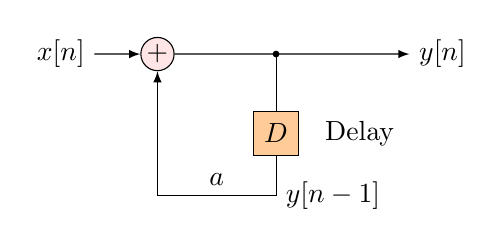
\begin{tikzpicture}
[
	scale=0.8,
	delay/.style={draw=black, fill=orange!40, minimum width=1.6em, minimum height=1.6em},
	adder/.style={circle, draw=black, fill=pink!40, minimum width=1.2em, minimum height=1.2em, inner sep=0},	
	br/.style={circle, draw=black, fill=black, minimum width=0.2em, minimum height=0.2em, inner sep=0},		
]

      \matrix (m) [row sep=5mm, column sep=10mm]{
      \node [adder] (m00) {$+$}; & \node[br] (m01)  {}; & \coordinate (m03) {} ;\\
       &\node [delay] (m11) {$D$};  &\\ 
        &  \coordinate (m22) {};  & \\
      };



%       \foreach \i/\j in {0/1, 1/3, 3/5, 5/7}
%     {
% 		\draw[-latex] (m\i 1) -- (m\j 1);
% 		\draw[-latex] (m\i 2) -- (m\j 2);				
%     }
% 
%       \foreach \i/\j in {0/2, 2/4, 4/5, 5/6}
%     {
% 		\draw[latex-] (m\i 0) -- (m\j 0);
% 		\draw[latex-] (m\i 3) -- (m\j 3);				
%     }
% 
% 
%    \draw[-latex] (m00) -- node[midway, above] {$1/a_0$} (m01);
%     \draw[-latex]  (m01) -- (m02);
%     \draw[-latex] (m02) -- node[midway, above] {$b_0$} (m03);
% % 
%     \draw[latex-] (m20)  -- node[midway, above] {$-a_1$} (m21);
%     \draw[-latex] (m22)  -- node[midway, above] {$b_1$} (m23);
%     
%     \draw[latex-] (m40)  -- node[midway, above] {$-a_2$} (m41);
%     \draw[-latex] (m42)  -- node[midway, above] {$b_2$} (m43);
%     
%     \draw[latex-] (m60)  -- node[midway, above] {$-a_{N-1}$} (m61);
%     \draw[-latex] (m62)  -- node[midway, above] {$b_{N-1}$} (m63);    
% 
% 	\draw[-latex] (m72) -- (m82) -- node[midway, above] {$b_{N}$} (m83)  -- (m63);
	\draw[-latex] (m01) -- (m11) (m11) -- (m22) -| (m00) node[near start, above] {$a$} ;
	\node at (m11) [anchor=west, xshift=5mm] {Delay};
	\node at (m22) [anchor=west] {$y[n-1]$};

	\draw[latex-] (m00) -- ++(-1,0) node[anchor=east] {$x[n]$};
	\draw[-latex] (m00) -- ++(4,0) node[anchor=west] {$y[n]$};
	%\draw[latex-] (m00) -- ++(-1,0);
\end{tikzpicture}
            \column{0.38\textwidth}
    \end{columns}
\end{frame}

\subsection{General block-Diagram Representation of the Recursive System}
\begin{frame}
    \begin{columns}
            \column{0.58\textwidth}
                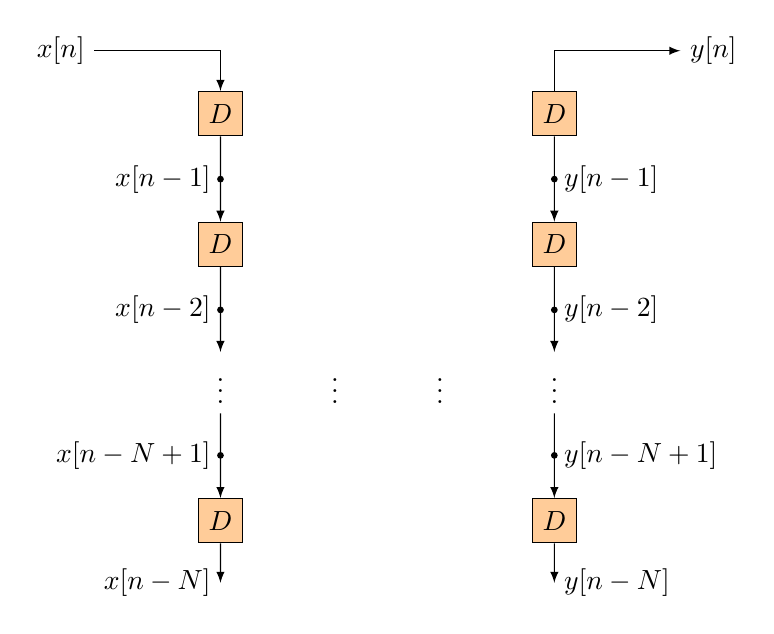
\begin{tikzpicture}
[
	scale=0.8,
	delay/.style={draw=black, fill=orange!40, minimum width=1.6em, minimum height=1.6em},
	adder/.style={circle, draw=black, fill=pink!40, minimum width=1.2em, minimum height=1.2em, inner sep=0},	
	br/.style={circle, draw=black, fill=black, minimum width=0.2em, minimum height=0.2em, inner sep=0},		
]

      \matrix (m) [row sep=5mm, column sep=10mm]{
      \node [delay] (m00) {$D$}; &  &  & \node [delay] (m03) {$D$}; \\
      \node [br] (m10) {}; &  & & \node [br] (m13) {};\\
      \node [delay] (m20) {$D$}; &  & & \node [delay] (m23) {$D$}; \\
      \node [br] (m30) {}; &   & & \node [br] (m33) {};\\
      \node [] (m40) {$\vdots$}; & \node [] (m41) {$\vdots$};   & \node [] (m42) {$\vdots$};  & \node [] (m43) {$\vdots$}; \\
      \node [br] (m50) {}; &  &    & \node [br] (m53) {};\\
      \node [delay] (m60) {$D$}; & &  & \node [delay] (m63) {$D$}; \\
      \coordinate (m70) {}; &   &   & \coordinate (m73) {};\\
      };


%
%
  

      \foreach \i/\j in {0/2, 2/4, 4/6}
    {
		\draw[-latex] (m\i 0) -- (m\j 0);
		\draw[-latex] (m\i 3) -- (m\j 3);		
    }


      \foreach \i/\j in {6/7}
    {
		\draw[-latex] (m\i 0) -- (m\j 0);
		\draw[-latex] (m\i 3) -- (m\j 3);		
    }

%     \draw[-latex] (m00) -- node[midway, above] {$b_0$} (m01);
%     \draw[-latex] (m02) -- node[midway, above] {$1/a_0$} (m03);
% 
     \draw (m10) node[anchor=east] {$x[n-1]$};
     \draw (m13) node[anchor=west] {$y[n-1]$};

    \draw (m30) node[anchor=east] {$x[n-2]$} ;
    \draw (m33)  node[anchor=west] {$y[n-2]$};

    \draw (m50) node[anchor=east] {$x[n-N + 1]$};
    \draw (m53)  node[anchor=west] {$y[n-N + 1]$};

    \draw (m70) node[anchor=east] {$x[n-N]$} ;
    \draw (m73)  node[anchor=west] {$y[n-N]$};

    \draw[latex-] (m00) |- ++(-2, 1) node[anchor=east] {$x[n]$};
    \draw[-latex] (m03) |- ++(2, 1) node[anchor=west] {$y[n]$};

    %\pause
    %\draw[-latex] (m01) -- node[midway, above] {$w[n]$} (m02);
\end{tikzpicture}
            \column{0.38\textwidth}
    \end{columns}
\end{frame}

\begin{frame}
    \begin{columns}[T]
            \column{0.68\textwidth}
                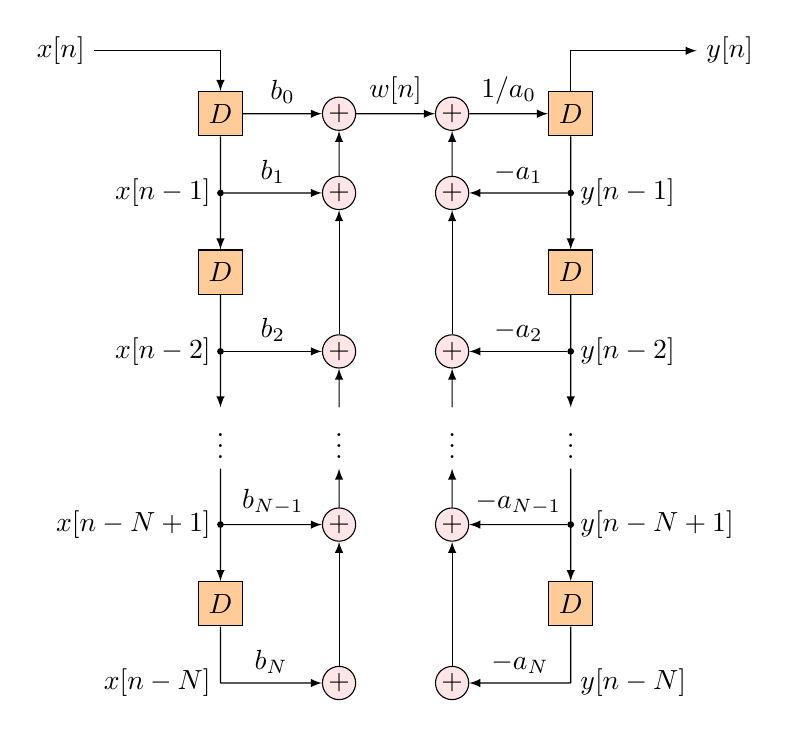
\begin{tikzpicture}
[
	scale=0.8,
	delay/.style={draw=black, fill=orange!40, minimum width=1.6em, minimum height=1.6em},
	adder/.style={circle, draw=black, fill=pink!40, minimum width=1.2em, minimum height=1.2em, inner sep=0},	
	br/.style={circle, draw=black, fill=black, minimum width=0.2em, minimum height=0.2em, inner sep=0},		
]

      \matrix (m) [row sep=5mm, column sep=10mm]{
      \node [delay] (m00) {$D$}; & \node[adder] (m01)  {$+$}; & \node[adder] (m02)  {$+$}; & \node [delay] (m03) {$D$}; \\
      \node [br] (m10) {}; & \node[adder] (m11)  {$+$};  & \node[adder] (m12)  {$+$};   & \node [br] (m13) {};\\
      \node [delay] (m20) {$D$}; &  & & \node [delay] (m23) {$D$}; \\
      \node [br] (m30) {}; & \node[adder] (m31)  {$+$};  & \node[adder] (m32)  {$+$};   & \node [br] (m33) {};\\
      \node [] (m40) {$\vdots$}; & \node [] (m41) {$\vdots$};   & \node [] (m42) {$\vdots$};  & \node [] (m43) {$\vdots$}; \\
      \node [br] (m50) {}; & \node[adder] (m51)  {$+$};  & \node[adder] (m52)  {$+$};   & \node [br] (m53) {};\\
      \node [delay] (m60) {$D$}; & &  & \node [delay] (m63) {$D$}; \\
      \coordinate (m70) {}; & \node[adder] (m71)  {$+$};  & \node[adder] (m72)  {$+$};   & \coordinate (m73) {};\\
      };


%
%
      \foreach \i/\j in {1/0, 3/1, 4/3, 5/4, 7/5}
    {
		\draw[-latex] (m\i 1) -- (m\j 1);
		\draw[-latex] (m\i 2) -- (m\j 2);		
    }

      \foreach \i/\j in {0/2, 2/4, 4/6}
    {
		\draw[-latex] (m\i 0) -- (m\j 0);
		\draw[-latex] (m\i 3) -- (m\j 3);		
    }


      \foreach \i/\j in {6/7}
    {
		\draw (m\i 0) -- (m\j 0);
		\draw (m\i 3) -- (m\j 3);		
    }

    \draw[-latex] (m00) -- node[midway, above] {$b_0$} (m01);
    \draw[-latex] (m02) -- node[midway, above] {$1/a_0$} (m03);

    \draw[-latex] (m10) node[anchor=east] {$x[n-1]$} -- node[midway, above] {$b_1$} (m11);
    \draw[latex-] (m12)  -- node[midway, above] {$-a_1$} (m13) node[anchor=west] {$y[n-1]$};

    \draw[-latex] (m30) node[anchor=east] {$x[n-2]$} -- node[midway, above] {$b_2$} (m31);
    \draw[latex-] (m32) -- node[midway, above] {$-a_2$} (m33)  node[anchor=west] {$y[n-2]$};

    \draw[-latex] (m50) node[anchor=east] {$x[n-N + 1]$}  -- node[midway, above] {$b_{N-1}$} (m51);
    \draw[latex-] (m52) -- node[midway, above] {$-a_{N-1}$} (m53)  node[anchor=west] {$y[n-N + 1]$};

    \draw[-latex] (m70) node[anchor=east] {$x[n-N]$}  -- node[midway, above] {$b_{N}$} (m71);
    \draw[latex-] (m72) -- node[midway, above] {$-a_{N}$} (m73)  node[anchor=west] {$y[n-N]$};

    \draw[latex-] (m00) |- ++(-2, 1) node[anchor=east] {$x[n]$};
    \draw[-latex] (m03) |- ++(2, 1) node[anchor=west] {$y[n]$};

    \pause
    \draw[-latex] (m01) -- node[midway, above] {$w[n]$} (m02);
\end{tikzpicture}

            \column{0.3\textwidth}
            \textbf{Direct form I implementation}\par
            This is a cascade of two linear systems. We can interchange the order of the two segments.
    \end{columns}
\end{frame}

\begin{frame}
    \begin{columns}
            \column{0.58\textwidth}
                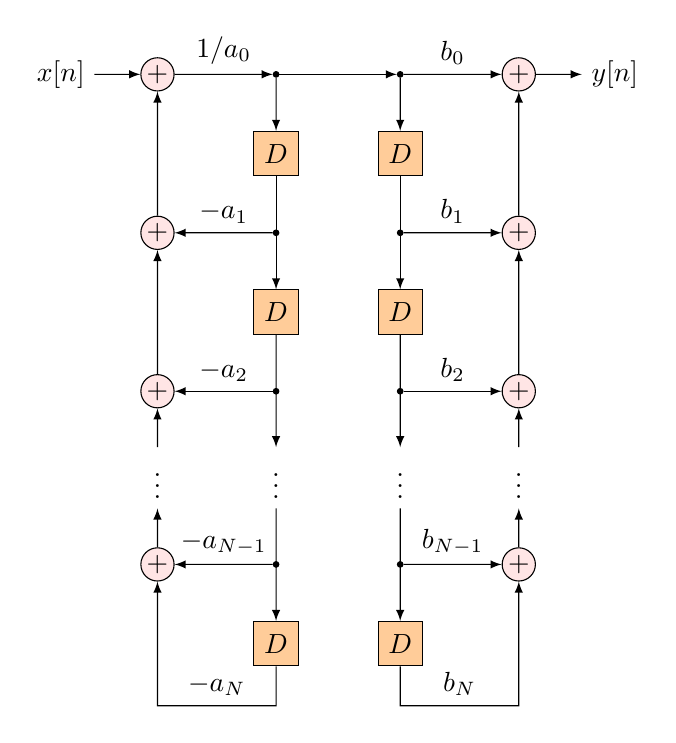
\begin{tikzpicture}
[
	scale=0.8,
	delay/.style={draw=black, fill=orange!40, minimum width=1.6em, minimum height=1.6em},
	adder/.style={circle, draw=black, fill=pink!40, minimum width=1.2em, minimum height=1.2em, inner sep=0},	
	br/.style={circle, draw=black, fill=black, minimum width=0.2em, minimum height=0.2em, inner sep=0},		
]

      \matrix (m) [row sep=5mm, column sep=10mm]{
      \node [adder] (m00) {$+$}; & \node[br] (m01)  {}; & \node[br] (m02)  {}; & \node [adder] (m03) {$+$}; \\
       &\node [delay] (m11) {$D$};  & \node [delay] (m12) {$D$}; &\\
       \node [adder] (m20) {$+$}; & \node[br] (m21)  {}; & \node[br] (m22)  {}; & \node [adder] (m23) {$+$}; \\
       &\node [delay] (m31) {$D$};  & \node [delay] (m32) {$D$}; &\\
       \node [adder] (m40) {$+$}; & \node[br] (m41)  {}; & \node[br] (m42)  {}; & \node [adder] (m43) {$+$}; \\
        \node [] (m50) {$\vdots$}; & \node [] (m51) {$\vdots$};   & \node [] (m52) {$\vdots$};  & \node [] (m53) {$\vdots$}; \\             
        \node [adder] (m60) {$+$}; & \node[br] (m61)  {}; & \node[br] (m62)  {}; & \node [adder] (m63) {$+$}; \\
       &\node [delay] (m71) {$D$};  & \node [delay] (m72) {$D$}; &\\       
       \coordinate  (m80) {}; & \coordinate[] (m81)  {}; & \coordinate[] (m82)  {}; & \coordinate [] (m83) {};\\     
% 
      };



      \foreach \i/\j in {0/1, 1/3, 3/5, 5/7}
    {
		\draw[-latex] (m\i 1) -- (m\j 1);
		\draw[-latex] (m\i 2) -- (m\j 2);				
    }

      \foreach \i/\j in {0/2, 2/4, 4/5, 5/6}
    {
		\draw[latex-] (m\i 0) -- (m\j 0);
		\draw[latex-] (m\i 3) -- (m\j 3);				
    }


   \draw[-latex] (m00) -- node[midway, above] {$1/a_0$} (m01);
    \draw[-latex]  (m01) -- (m02);
    \draw[-latex] (m02) -- node[midway, above] {$b_0$} (m03);
% 
    \draw[latex-] (m20)  -- node[midway, above] {$-a_1$} (m21);
    \draw[-latex] (m22)  -- node[midway, above] {$b_1$} (m23);
    
    \draw[latex-] (m40)  -- node[midway, above] {$-a_2$} (m41);
    \draw[-latex] (m42)  -- node[midway, above] {$b_2$} (m43);
    
    \draw[latex-] (m60)  -- node[midway, above] {$-a_{N-1}$} (m61);
    \draw[-latex] (m62)  -- node[midway, above] {$b_{N-1}$} (m63);    

	\draw[-latex] (m72) -- (m82) -- node[midway, above] {$b_{N}$} (m83)  -- (m63);
	\draw[latex-] (m60) -- (m80) -- node[midway, above] {$-a_{N}$} (m81)  -- (m71);

	\draw[latex-] (m00) -- ++(-1,0) node[anchor=east] {$x[n]$};
	\draw[-latex] (m03) -- ++(1,0) node[anchor=west] {$y[n]$};
	%\draw[latex-] (m00) -- ++(-1,0);
\end{tikzpicture}

            \column{0.38\textwidth}
    \end{columns}
\end{frame}

\begin{frame}
\mode<beamer>
{
    \begin{columns}[T]
            \column{0.68\textwidth}
                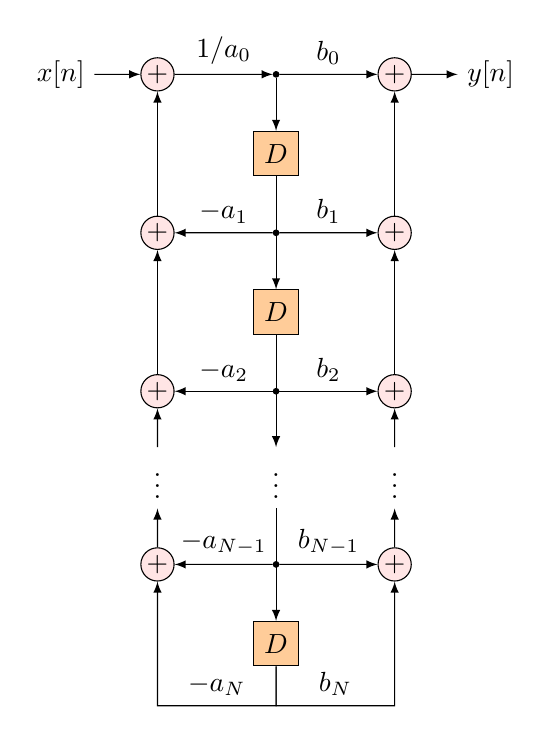
\begin{tikzpicture}
[
	scale=0.8,
	delay/.style={draw=black, fill=orange!40, minimum width=1.6em, minimum height=1.6em},
	adder/.style={circle, draw=black, fill=pink!40, minimum width=1.2em, minimum height=1.2em, inner sep=0},	
	br/.style={circle, draw=black, fill=black, minimum width=0.2em, minimum height=0.2em, inner sep=0},		
]

      \matrix (m) [row sep=5mm, column sep=10mm]{
      \node [adder] (m00) {$+$}; & \node[br] (m01)  {}; & \node [adder] (m03) {$+$}; \\
       &\node [delay] (m11) {$D$}; \\
       \node [adder] (m20) {$+$}; & \node[br] (m21)  {}; & \node [adder] (m23) {$+$}; \\
       &\node [delay] (m31) {$D$};  & \\
       \node [adder] (m40) {$+$}; & \node[br] (m41)  {}; & \node [adder] (m43) {$+$}; \\
        \node [] (m50) {$\vdots$}; & \node [] (m51) {$\vdots$};  & \node [] (m53) {$\vdots$}; \\             
        \node [adder] (m60) {$+$}; & \node[br] (m61)  {}; & \node [adder] (m63) {$+$}; \\
       &\node [delay] (m71) {$D$}; \\       
       \coordinate  (m80) {}; & \coordinate[] (m81)  {}; & \coordinate [] (m83) {};\\     
% 
      };



      \foreach \i/\j in {0/1, 1/3, 3/5, 5/7}
    {
		\draw[-latex] (m\i 1) -- (m\j 1);
			
    }
% 
      \foreach \i/\j in {0/2, 2/4, 4/5, 5/6}
    {
		\draw[latex-] (m\i 0) -- (m\j 0);
		\draw[latex-] (m\i 3) -- (m\j 3);				
    }
% 
% 
   \draw[-latex] (m00) -- node[midway, above] {$1/a_0$} (m01);
    \draw[-latex] (m01) -- node[midway, above] {$b_0$} (m03);
% 
    \draw[latex-] (m20)  -- node[midway, above] {$-a_1$} (m21);
    \draw[-latex] (m21)  -- node[midway, above] {$b_1$} (m23);
    
    \draw[latex-] (m40)  -- node[midway, above] {$-a_2$} (m41);
    \draw[-latex] (m41)  -- node[midway, above] {$b_2$} (m43);
%     
    \draw[latex-] (m60)  -- node[midway, above] {$-a_{N-1}$} (m61);
    \draw[-latex] (m61)  -- node[midway, above] {$b_{N-1}$} (m63);    
% 
	\draw[-latex] (m71) -- (m81) -- node[midway, above] {$b_{N}$} (m83)  -- (m63);
	\draw[latex-] (m60) -- (m80) -- node[midway, above] {$-a_{N}$} (m81)  -- (m71);

	\draw[latex-] (m00) -- ++(-1,0) node[anchor=east] {$x[n]$};
	\draw[-latex] (m03) -- ++(1,0) node[anchor=west] {$y[n]$};

\end{tikzpicture}

            \column{0.3\textwidth}
            Result of combining the two chains of delays.\par
            \textbf{Direct form II implementation}
    \end{columns}
    }
\end{frame}

\section{Revisiting Fourier Series}
\begin{frame}{Convolution}
    \begin{enumerate}
      \item In representing and analyzing LTI systems, our approach has been to decompose the system inputs into a liner combination of basic signals and exploit the fact that for a linear system, the response is the same linear combination of the responses to the basic inputs.
      \item The convolution sum and the convolution integral req out of the particular choice of the basic signals, delayed unit impulses.
      \item This choice has the advantage that for systems that are time invariant in addition to being linear, once the response to an impulse at one time position is known, then the response id know at all time positions.
    \end{enumerate}
\end{frame}

\begin{frame}{Complex Exponentials with Unity Magnitude as Basic Signals}
    \begin{enumerate}
      \item When we select complex exponential with unity magnitude as the basic signals, the decomposition of this form of a periodic signal is the Fourier series.
      \item For aperiodic signals, it becomes the Fourier transform.
      \item In latter lectures, we will generalize this representation to Laplace tangram for continuous-time signals and $z$-transform for discrete-time signals.
    \end{enumerate}
\end{frame}

\begin{frame}[plain]
    \begin{columns}
            \column{0.48\textwidth}
                Consider a linear system
                {
                \tikzstyle{int}=[draw, fill=pink!60, minimum size=2em]
\tikzstyle{init} = [pin edge={to-,thin,black}]

\begin{tikzpicture}[node distance=2.5cm,auto,>=latex']
	
	\begin{scope}[yshift=-2cm,
		start chain,
		node distance=5mm,
		every node/.style={int, draw,on chain,join,inner sep=2mm},
		every join/.style={->}
		]
		\node[draw=none, fill=none]  {$u[n]$};	
		\node { $h[n]$};
		\node[draw=none, fill=none]   {$s[n]$};
	\end{scope}
	
	
\end{tikzpicture} \par
                }
                If
                \begin{equation*}
                    x(t) = a_1\phi_1(t) + a_2\phi_2(t) + \cdots
                \end{equation*}
                and
                \begin{equation*}
                    \phi_k(t) \longrightarrow \psi_k(t), \quad \text{(output due to $\phi_k(t) $)}
                \end{equation*}
                then
                \pause
                \begin{equation*}
                    y(t) = a_1\psi_1(t) + a_2\psi_2(t) + \cdots
                \end{equation*}
                Identical for DT. So
                \pause
                \begin{align*}
                   \text{If}\quad x(t) &= a_1\phi_1 + a_2\phi_2 + \cdots,\\
                   \text{then}\quad y(t) &= a_1\psi_1 + a_2\psi_2 + \cdots.
                \end{align*}

                \pause
            \column{0.48\textwidth}
                Choose $\phi_k(t)$ or $\phi_k[n]$ so that
                \begin{enumerate}
                    \item A broad class of signals can be constructed as a linear combination of $\phi_k$s
                    \item Response to $\phi_k$s easy to compute.
                \end{enumerate}
                \pause
                Choice of signals $\delta(t-k\Delta)$ and $\delta[n-k]$ lead to the convolution integral and convolution sum.
                \begin{align*}
                    \text{CT}\quad \phi_k(t) &=  \delta(t-k\Delta)\\
                    \psi_k(t) &= h(t-k\Delta)\quad \Rightarrow \text{ convolution integral}\\
                    \text{DT}\quad \phi_k[n] &=  \delta[n-k]\\
                    \psi_k[n] &= h[n-k]\quad \Rightarrow \text{ convolution sum}
                \end{align*}
                \pause
                Here, we  choose complex exponentials as the set of basic signals.
                \begin{align*}
                    \phi_k(t) &= e^{s_k t},\quad s_k \text{ complex}\\
                    \phi_k[n] &= z_k^n,\quad z_k \text{ complex}\\
                \end{align*}

    \end{columns}
\end{frame}

\begin{frame}{Fourier Analysis}
\begin{align*}
  \text{CT}\quad s_k &= j\omega k\quad \text{purely imaginary} \quad \phi_k(t) &= e^{j\omega_k t}\\
  \text{DT}\quad |z_k| &= 1\quad \text{} \quad \phi_k[n] &= e^{j\omega_k n}\\
\end{align*}
$s_k$ complex $\Rightarrow$  Laplace transfrom\par
$z_k$ complex $\Rightarrow$ $z$-transform

\end{frame}

\begin{frame}{Eigenfunction Property}
    Consider $\phi_k(t) = e^{j\omega_k t}$:
    \begin{equation*}
        e^{j\omega_k t} \longrightarrow H(\omega_k) e^{j\omega_k t} \quad \text{(a scaled-version of the input)}
    \end{equation*}
    \textbf{``Proof'':}\pause
    \mode<beamer>
    {
        \begin{equation*}
            e^{j\omega_k t} \longrightarrow \int_{-\infty}^{\infty}h(\tau)e^{j\omega_k (t-\tau)}d\tau
        \end{equation*}
        \pause
        \begin{equation*}
            e^{j\omega_k t} \longrightarrow
            \underset{\mathclap{\tikz \node {$\uparrow$} node [below=3ex, text=red] {eigenfunction};}}{
            e^{j\omega_k t}
            }
            \underbrace{
            \int_{-\infty}^{\infty} h(\tau)e^{-j\omega_k \tau}d\tau
            }_{\textcolor{red}{\text{eigenvalue}}}
        \end{equation*}
    }
\end{frame}


\begin{frame}{CT Fourier Series}
    \begin{columns}
        \column{0.48\textwidth}
            \begin{equation*}
                x(t) = x(t+T), \quad T = \text{ period},  \quad\omega_0 = \frac{2\pi}{T}
            \end{equation*}
            Consider the periodic exponential signal with the same fundamental period:
            \begin{align*}
                e^{j\omega_0 t},  & \quad T = \frac{2\pi}{\omega_0}\\
                e^{jk\omega_0 t},  &\quad  T = \frac{2\pi}{k\omega_0},  \quad \text{harmonically related}
            \end{align*}
            \begin{equation*}
                \text{Fourier series:}\quad  x(t) = \sum_{k=-\infty}^{\infty}a_k e^{jk\omega_0 t}
            \end{equation*}
            \pause
            \begin{enumerate}
              \item How do we find $a_k$s?
              \item What are the signal that can be expressed in this form? [already answered, see convergence]
            \end{enumerate}
        \column{0.48\textwidth}
            \mode<beamer>
            {
            \begin{equation*}
                \int_{T}e^{jm\omega_0t}dt = \begin{cases}T, & m=0,\\0, &m\neq 0.\end{cases}
            \end{equation*}
            \pause
            \begin{equation*}
                \begin{array}{ccc}
                    \int_{T}e^{jm\omega_0t}dt &= \int_{T}\cos m\omega_0 t dt &+  j\int_{T}\sin m\omega_0 t dt\\
                    m\neq 0 & 0 & 0\\
                    m = 0 & T & 0
                \end{array}
            \end{equation*}
            \pause
            Start with the \fs~ equation
            \begin{equation*}
                x(t) = \sum_{k=-\infty}^{\infty}a_k e^{jk\omega_0 t}
            \end{equation*}
            Multiplying both sides by $e^{-jn\omega_0t}$
            \begin{equation*}
                x(t)e^{-jn\omega_0t} = \sum_{k=-\infty}^{\infty}a_k e^{jk\omega_0 t}e^{-jn\omega_0t}
            \end{equation*}
            Integrating over one period
            \begin{equation*}
                \int_{T}x(t)e^{-jn\omega_0t} = \int_{T}\sum_{k=-\infty}^{\infty}a_k e^{jk\omega_0 t}e^{-jn\omega_0t}
            \end{equation*}

            }

    \end{columns}


\end{frame}


\begin{frame}[plain]
    \begin{columns}
        \column{0.48\textwidth}
            \mode<beamer>
            {
                Integrating over one period
                \begin{equation*}
                    \int_{T}x(t)e^{-jn\omega_0t}dt = \int_{T}\sum_{k=-\infty}^{\infty}a_k e^{jk\omega_0 t}e^{-jn\omega_0t}dt
                \end{equation*}
                \pause
                \begin{equation*}
                    \int_{T}x(t)e^{-jn\omega_0t}dt = \sum_{k=-\infty}^{\infty}a_k \int_{T} \left[e^{j(k-n)\omega_0 t}\right]dt
                \end{equation*}
                \pause
                \begin{equation*}
                    \int_{T} e^{j(k-n)\omega_0 t} dt = \begin{cases}T, & k = n,\\ 0, & k \neq n.\\\end{cases}
                \end{equation*}
                \pause
                \begin{equation*}
                    a_n = \frac{1}{T}\int_{T} x(t) e^{-jn\omega_0 t}dt
                \end{equation*}
                So
                \pause
                \begin{equation*}
                    a_k = \frac{1}{T}\int_{T} x(t) e^{-jk\omega_0 t}dt
                \end{equation*}


            }
        \column{0.48\textwidth}
            \mode<beamer>
            {



            }

    \end{columns}
\end{frame}


%\begin{frame}{}
%    \begin{enumerate}
%        \item
%    \end{enumerate}
%
%    \mode<beamer>
%    {
%        \begin{columns}
%            \column{0.48\textwidth}
%            \column{0.48\textwidth}
%        \end{columns}
%    }
%\end{frame} 


%\begin{frame}{}
%    \begin{enumerate}
%        \item
%    \end{enumerate}
%
%    \mode<beamer>
%    {
%        \begin{columns}
%            \column{0.48\textwidth}
%            \column{0.48\textwidth}
%        \end{columns}
%    }
%\end{frame}

%\begin{figure}
%    \centering
%    \input{figures/sys_for_operational_def}
%    \caption{}\label{fi:sys_for_operational_def}
%\end{figure}


%\begin{figure}
%    \centering
%    \input{figures/sys_for_operational_def}
%    \caption{}\label{fi:sys_for_operational_def}
%\end{figure}

%\begin{frame}{}
%    \begin{enumerate}
%        \item
%    \end{enumerate}
%
%    \mode<beamer>
%    {
%        \begin{columns}
%            \column{0.48\textwidth}
%            \column{0.48\textwidth}
%        \end{columns}
%    }
%\end{frame}

%\begin{figure}
%    \centering
%    \input{figures/sys_for_operational_def}
%    \caption{}\label{fi:sys_for_operational_def}
%\end{figure}
